%%    _____  _____
%%   |  __ \|  __ \    AUTHOR: Pedro Rivero
%%   | |__) | |__) |   ---------------------------------
%%   |  ___/|  _  /    DATE: June 20, 2020
%%   | |    | | \ \    ---------------------------------
%%   |_|    |_|  \_\   https://github.com/pedrorrivero
%%

\documentclass[9pt, aspectratio=169]{beamer}
% \documentclass[9pt, handout, aspectratio=169]{beamer}	% Skip \pause commands
\usetheme{PRRwide}
\usepackage{PRRmath}

% \setbeameroption{show notes}
% \setbeameroption{show only notes}

%% ----------------------------------------------------------------------------
%% FRONT-MATTER
%% ----------------------------------------------------------------------------

\title{Quantum Computation for the Understanding of Mass}
\subtitle{Simulating Quantum Field Theories}
\author{Pedro Rivero}
\institute{Argonne National Laboratory \\ Illinois Institute of Technology}
\newcommand{\mail}{priveroramirez@anl.gov}
\date{\today}
\newcommand{\website}{
	\href{https://www.phy.anl.gov}
	{www.phy.anl.gov}
}

\begin{document}
	\justify
	\setlength{\abovedisplayskip}{0pt}
	\setlength{\belowdisplayskip}{12pt}
	\setlength{\abovedisplayshortskip}{0pt}
	\setlength{\belowdisplayshortskip}{12pt}

\begin{frame}[plain,t]
	\titlepage
\end{frame}

\begin{frame}[c]{Contents}
%		\begin{multicols}{2}
%  			\tableofcontents
%		\end{multicols}
	\tableofcontents
\end{frame}


%% ----------------------------------------------------------------------------
%% MAIN-MATTER
%% ----------------------------------------------------------------------------

\section{Introduction}

\begin{frame}{Introduction}

	\begin{multicols}{2}

		\begin{itemize}
			\item<2-> Quantum Chromodynamics (QCD) is the theory of the strong nuclear force, and it holds many mysteries such as \textbf{mass generation}.
			\item<2-> QCD is currently studied using brute-force numerics on the world’s largest supercomputers, nonetheless many of its aspects cannot be reproduced by classical means.
			\item<3-> The \textbf{NJL model} is an effective field theory regarded as a low-energy approximation to QCD. It retains certain key features like the so called Goldstone modes, and \textbf{dynamical chiral symmetry breaking}; and can also be solved nonperturbatively for verification.
		\end{itemize}

		\begin{center}
			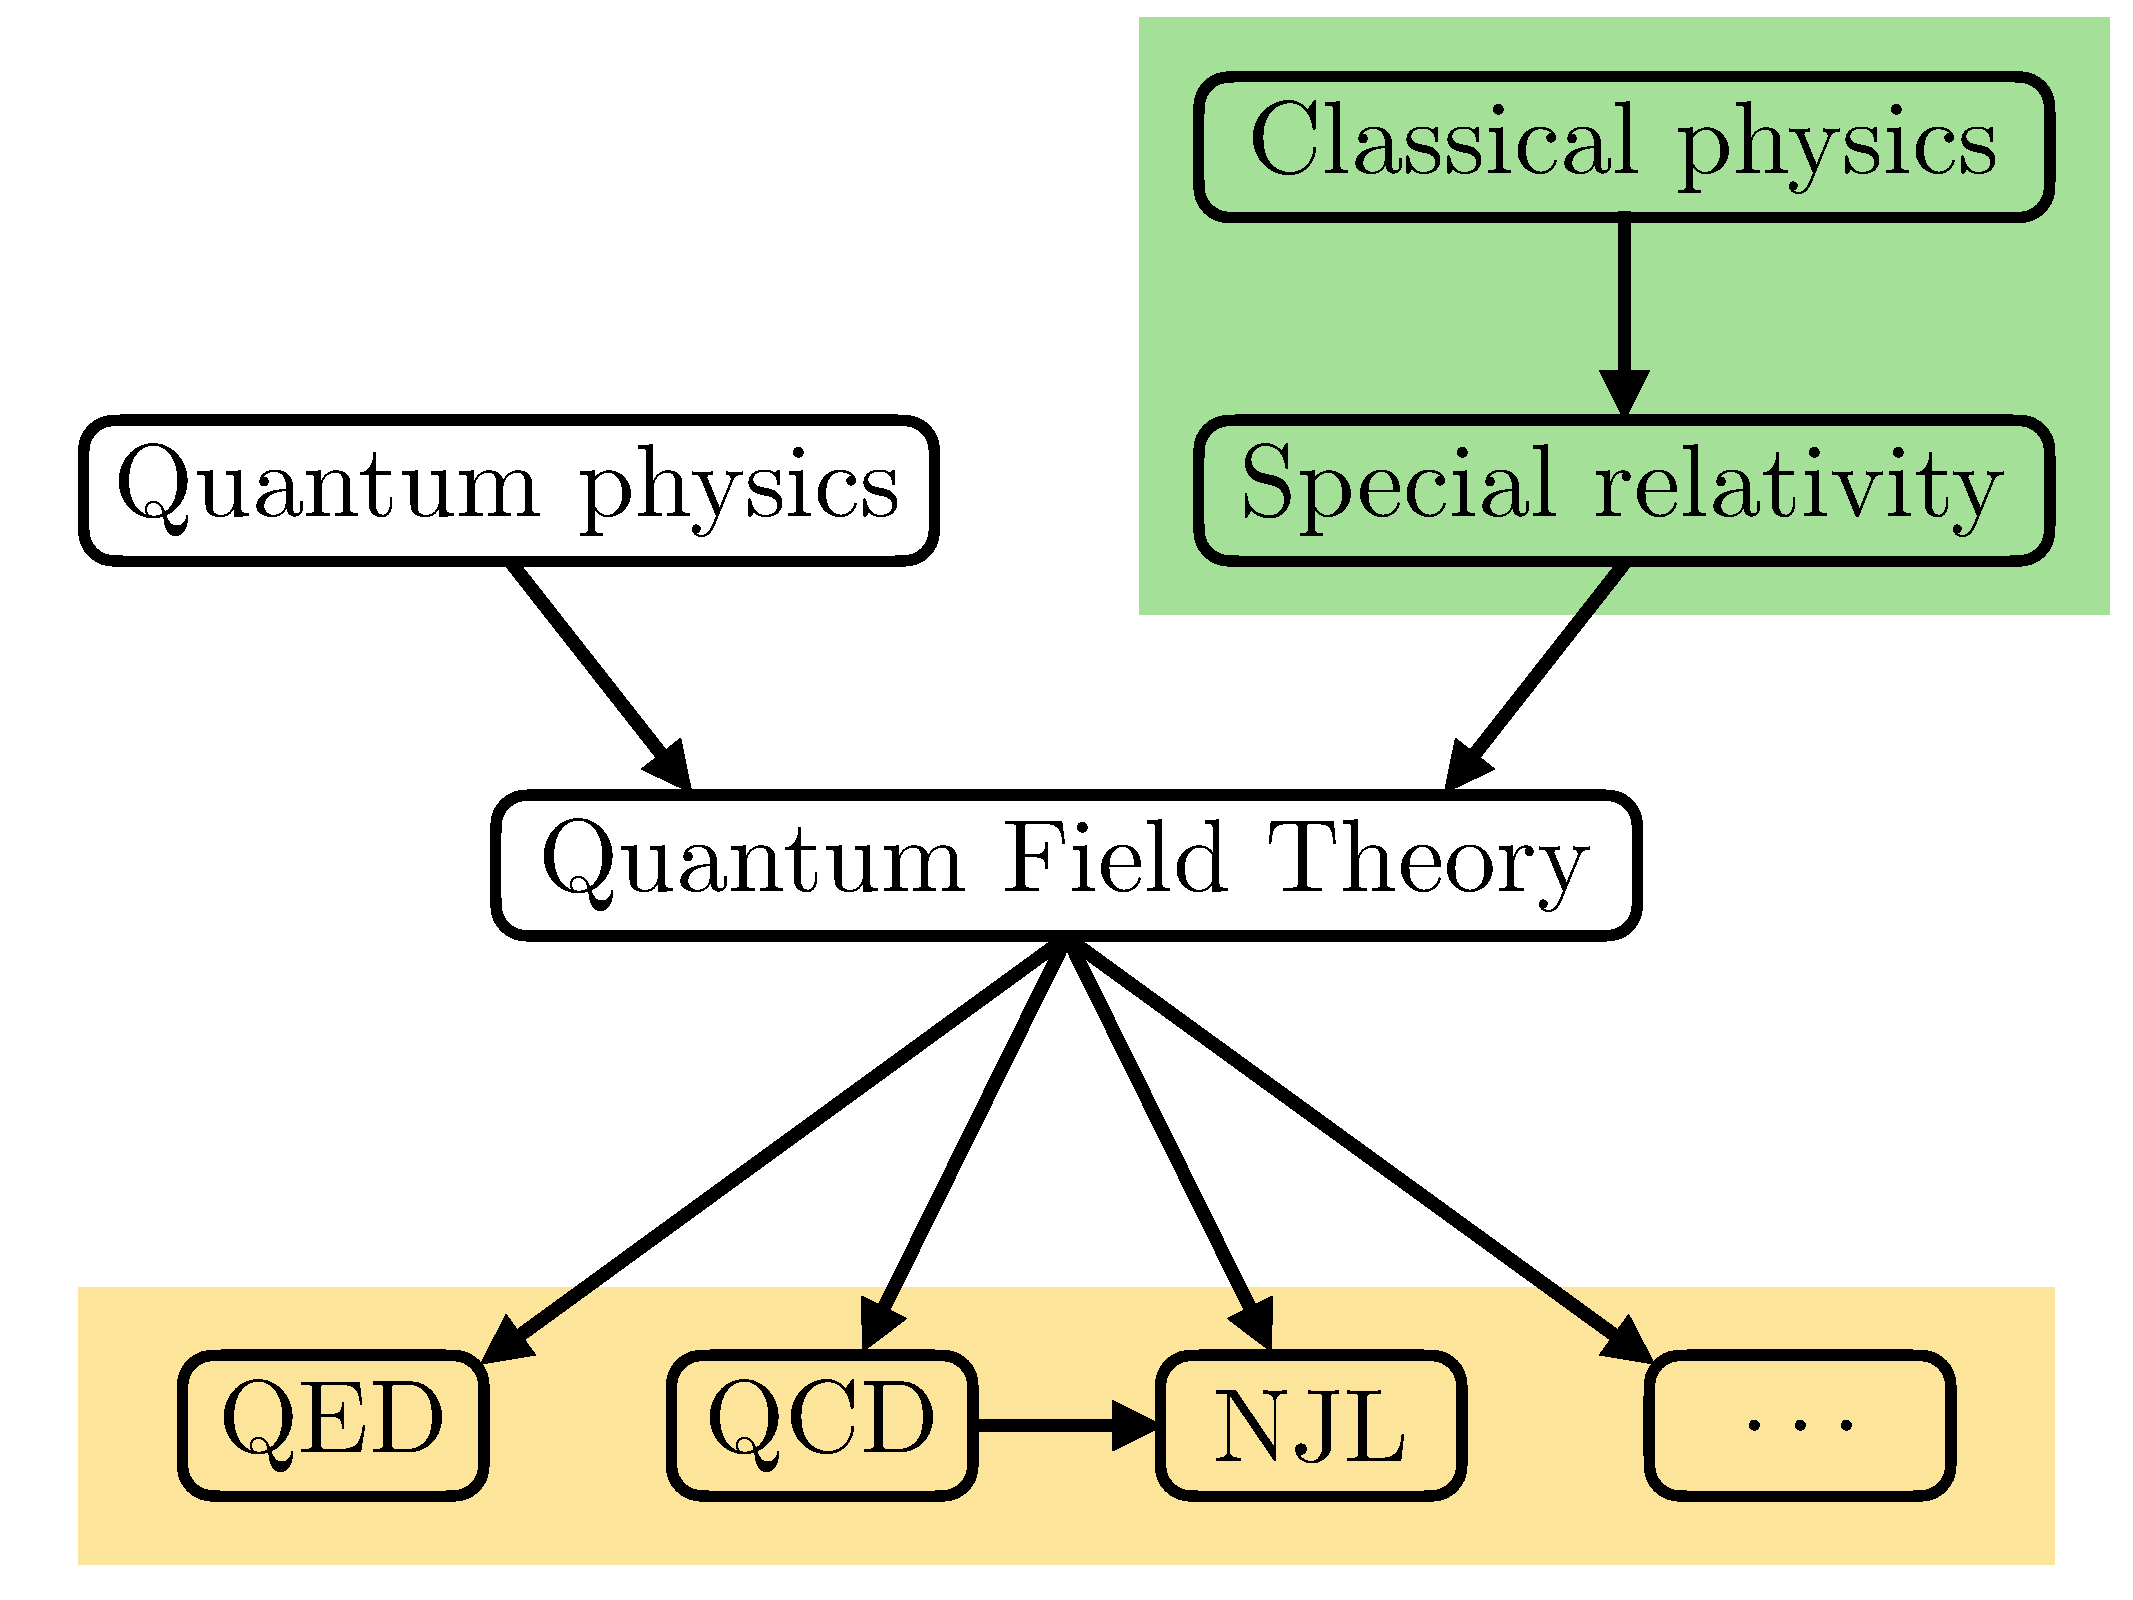
\includegraphics[width=.40\paperwidth]{Figures/quantum-field-theory}
		\end{center}

	\end{multicols}

\end{frame}

%% ----------------------------------------------------------------------------

\subsection{NJL model and the gap equation}

\begin{frame}{NJL model and the gap equation}

	\begin{multicols}{2}

		\begin{center}
			\underline{\textbf{NJL LAGRANGIAN DENSITY}}\\
			\small{\emph{Simplest version that reproduces a condensate}}
			\begin{gather*}
				\vspace{0.4em}
				\mathcal{L}(x) \defeq
			    \bar{\psi}(x) \qty(i\slashed{\partial}-m) \psi(x) + \mathcal{L}_{I}(x)
					\\[10pt]
				\mathcal{L}_{I}(x) =
			    \frac{1}{2} G_{\pi} \qty[\bar{\psi}(x)\psi(x)]^2
			\end{gather*}
		\end{center}

		\columnbreak

		\begin{center}
			\underline{\textbf{NJL HAMILTONIAN DENSITY}}\\
			\small{\emph{Obtained through the Lengendre transform}}
			\begin{gather*}
				\vspace{-1em}
			  \mathcal{H}(x) \defeq
			    \bar{\psi}(x)\qty(m - i\gamma^{1}\partial_{1})\psi(x) + \mathcal{H}_{I}(x) \\[8pt]
				\mathcal{H}_{I}(x) =
		    	- \frac{1}{2} G_{\pi} \qty[\bar{\psi}(x)\psi(x)]^{2}
			\end{gather*}
		\end{center}

	\end{multicols}

	\vspace{1em} \pause

	The \textbf{bare and dressed masses} appear on the bare quark propagator $S_{0}$, and the NJL dressed quark propagator $S$ respectively. We can find a relationship between these two by solving the \textbf{gap equation}:

	\begin{gather*}
		S^{-1} =
			S_{0}^{-1} - 2iG_{\pi} \int \frac{\dd[2]{p}}{\qty(2\pi)^{2}}
			N_\text{color} N_\text{flavor} \text{Tr}_\text{\tiny{D}}\qty[S] \\
	  M \simeq
	    m + 4iG_\pi N_\text{color} N_\text{flavor}
	    \int \frac{\dd[2]{p}}{(2\pi)^2} \frac{M}{p^2 - M^2}
	\end{gather*}

\end{frame}

%% ----------------------------------------------------------------------------

\subsection{Mass generation}

\begin{frame}{Mass generation}

	\begin{center}
		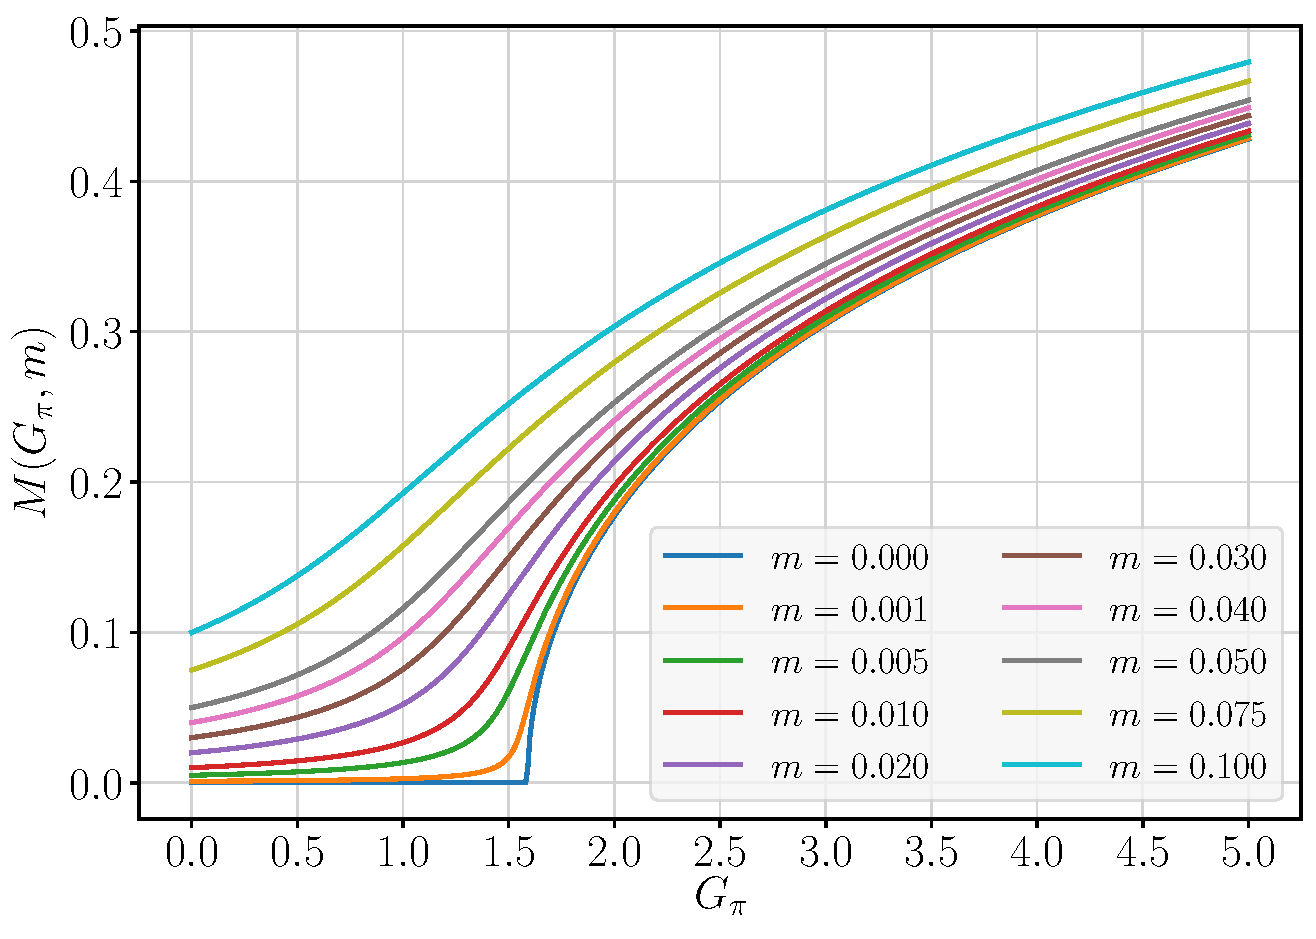
\includegraphics[width=.5\paperwidth]{Figures/NJL1-model-solving/NJL1-dressed-mass-curves}
	\end{center}

	\vspace{-1em}

	\begin{table}[!bp]
	  \centering
	  % \caption{Parameters used for solving the NJL model in $1+1$ dimensions.}
	  \label{tab:NJL1-analytical-solution-parameters}
	  \begin{tabular}{ c c c c c }
	    \hline
	    % \rule{0pt}{14pt}
	    $N_\text{Dirac}$ & $N_\text{color}$ & $N_\text{flavor}$ &
	    $\Lambda_{IR}$ & $\Lambda_{UV}$ \\
	    \hline
	    \hline
	    % \rule{0pt}{14pt}
	    $1+1 \ra 2$ & $1$ & $1$ & $0.240$ GeV & $0.645$ GeV \\
	    \hline
	  \end{tabular}
	\end{table}

\end{frame}


%% ----------------------------------------------------------------------------

% \begin{frame}[c]{Contents}
% %		\begin{multicols}{2}
% %  			\tableofcontents
% %		\end{multicols}
% 	\tableofcontents
% \end{frame}

%% ----------------------------------------------------------------------------
%% ----------------------------------------------------------------------------

\section{Quantum computing formulation of the NJL model}

\begin{frame}{NJL Hamiltonian in $1+1$ dimensions}

	We can define the Hamiltonian of the system as the integral over space of the Hamiltonian density:

	\begin{gather*}
	  H = \int \mathcal{H}(x) \dd{x}
	    = \int \qty{\bar{\psi}(x)\qty(m-i\gamma^{1}\partial_{1})\psi(x) -
	                \frac{1}{2}G_{\pi}\qty[\bar{\psi}(x)\psi(x)]^{2}} \dd{x}
	\end{gather*}

	\pause

	For a basis where:

	\begin{gather*}
		\psi = \mqty[\psi_{+} \\ \psi_{-}] \qc
	  \bar{\psi} \defeq \psi^{\dagger}\gamma^{0} \qc
		\gamma^{0} = \mqty[1 & 0\\ 0 & -1] \qc
	  \gamma^{1} = \mqty[0 & -1\\ 1 & 0]
	\end{gather*}

	We can write the kinetic term as:

	\begin{gather*}
	  \bar{\psi}\qty(-i\gamma^{1}\partial_{1})\psi =
			\frac{i}{2} \qty{
	      \qty[ \psi^{\dagger}_{+} \qty(\partial_{1}\psi_{-}) -
	      \qty(\partial_{1}\psi^{\dagger}_{+}) \psi_{-} ] +
	      \qty[ \psi^{\dagger}_{-} \qty(\partial_{1}\psi_{+}) -
	      \qty(\partial_{1}\psi^{\dagger}_{-}) \psi_{+} ]
	    }
	\end{gather*}

\end{frame}

%% ----------------------------------------------------------------------------

\subsection{Lattice formulation}

\begin{frame}[allowframebreaks]{Lattice formulation}

	The two groups in brackets are essentially equivalent to one another by virtue of exchanging positive and negative energy components. This is the motivation behind \textbf{staggered fermion lattices}, which use two computational lattice sites for each theoretical value of $\psi$. These newly defined operators obey the \textbf{canonical commutation relations for fermions}.

	\vspace{1em}

	\begin{figure}[!tbp]
		\centering
		\begin{minipage}[c]{.45\linewidth}
			\centering
			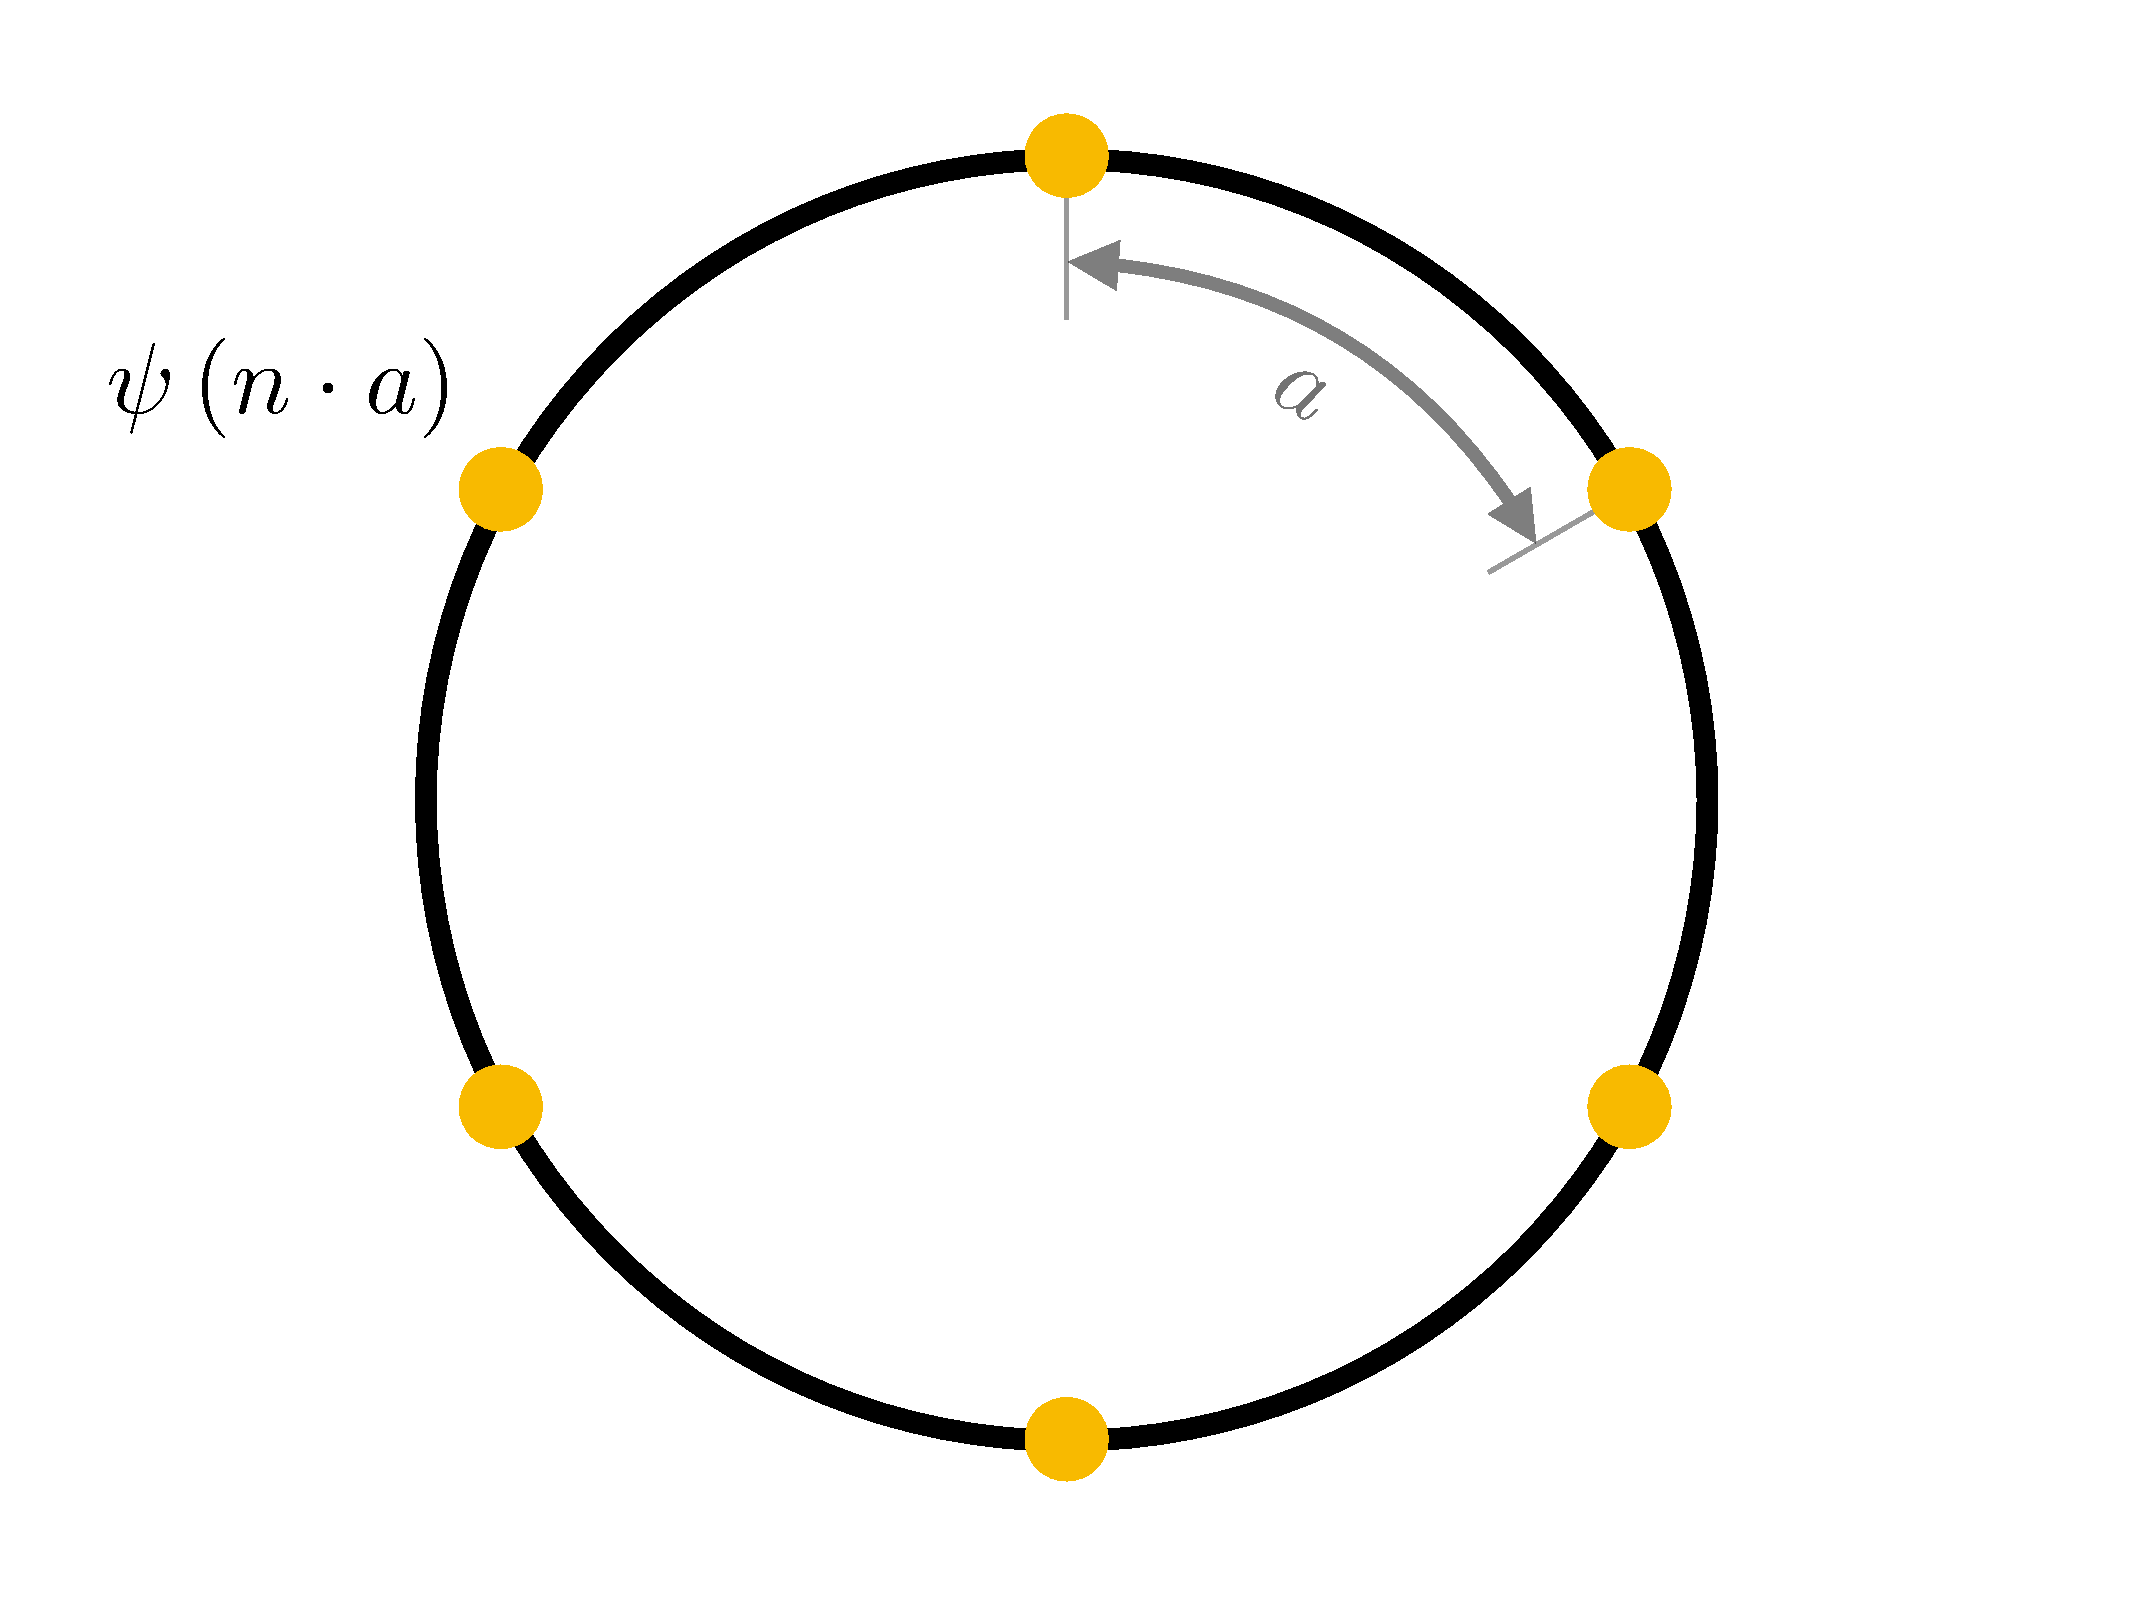
\includegraphics[width=\linewidth]{Figures/NJL1-model-solving/theoretical-fermion-lattice}
		\end{minipage}
	  \hspace{.025\linewidth}
		\begin{minipage}[c]{.45\linewidth}
			\centering
			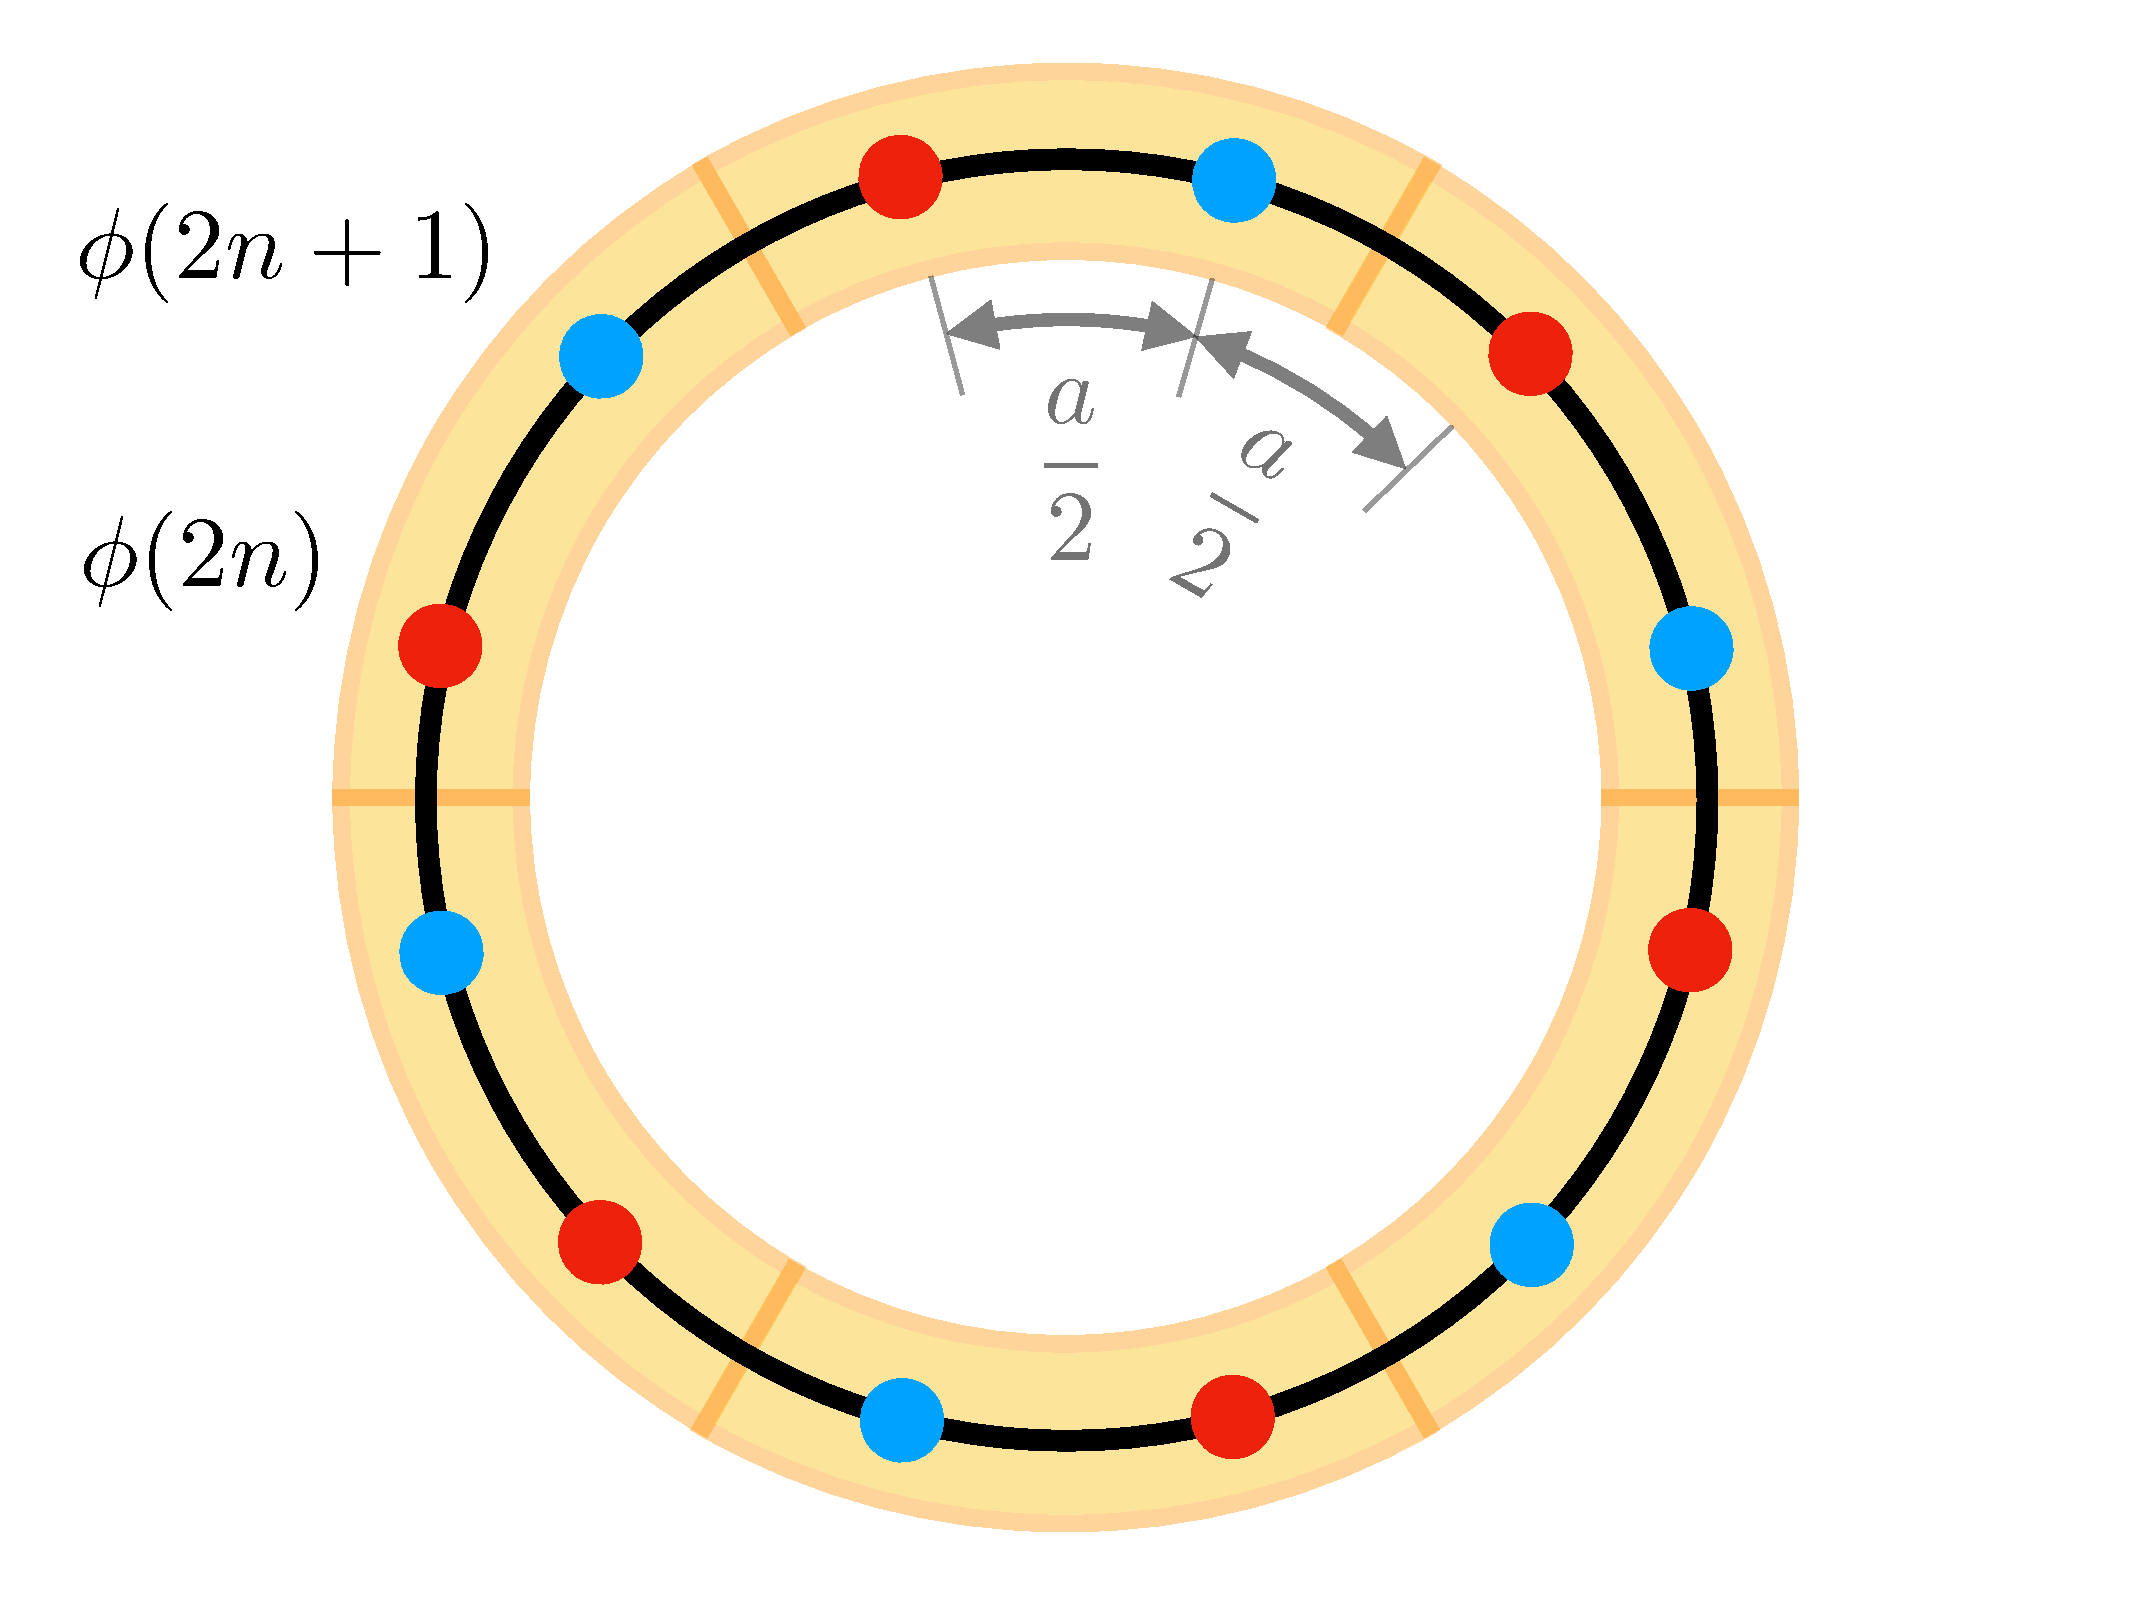
\includegraphics[width=\linewidth]{Figures/NJL1-model-solving/computational-fermion-lattice}
		\end{minipage}
		% \caption{Representations of a fermion lattice in $1+1$ dimensions, with periodic boundary conditions, and for $N=6$ theoretical lattice sites. (Left) Theoretical lattice. (Right) Staggered computational lattice.}
	  % \label{fig:staggered-fermion-lattice}
	\end{figure}

\break

	And it is now straight forward to obtain all other components of the Hamiltonian from the expressions in the Hamiltonian density, which are written in terms of \textbf{Dirac bilinears}.

	\vspace{1em}

	\begin{gather*}
	  H_{N} = H_{N}^{(M)} + H_{N}^{(K)} + H_{N}^{(I)}
	    \label{eq:NJL1-staggered-discretization} \\[10pt]
	  H_{N}^{(M)} =
	    m \sum_{n=0}^{2N-1} (-1)^{n}\phi^{\dagger}(n)\phi(n) \\
	  H_{N}^{(K)} =
	    \frac{i}{a} \sum_{n=0}^{2N-1} \qty[
	    \phi^{\dagger}(n)\phi(n+1) - \phi^{\dagger}(n+1)\phi(n)] \\
	  H_{N}^{(I)} =
	    - \frac{1}{2a} G_{\pi} \sum_{n=0}^{N-1} \qty[
	      \phi^{\dagger}(2n)\phi(2n) - \phi^{\dagger}(2n+1)\phi(2n+1)
	    ]^{2}
	\end{gather*}

\end{frame}

%% ----------------------------------------------------------------------------

\subsection{Fermion-qubit mapping}

\begin{frame}{Fermion-qubit mapping}

	Generally speaking, quantum computers cannot measure any given operator directly. Therefore, in order to simulate any Hamiltonian in a quantum processor, one needs to efficiently map its component operators onto ones suitable for evaluation in such machines (e.g. \textbf{Pauli operators} and the identity).

	\medskip \pause

	In one spatial dimension, spin-$\frac{1}{2}$ particles (i.e. qubits) behave much like fermions. The \textbf{Jordan-Wigner transform} associates spin \emph{down/up} with \emph{occupied/unoccupied} fermion states:

	\begin{align*}
		\ket{\ua} \cong \ket{0} &\qc
			\ket{\da} \cong \ket{1} \\
    \ket{\da} \cong \phi^{\dagger}\ket{0} &\qc
			\ket{\ua} \cong \phi\ket{1} \\[5pt]
			S(n)\phi(n) \ra \sigma^{+}(n) &\qc
			\phi^{\dagger}(n)S^{\dagger}(n) \ra \sigma^{-}(n)
	\end{align*}

	\pause

	Particularly, choosing a gauge which makes the \textbf{string operator} $S(n)$ hermitian $\forall n$:

	\begin{gather*}
		\phi(n) \ra \qty[\prod_{l<n} \sigma^3(l)]\sigma^{+}(n) \qc
		\phi^{\dagger}(n) \ra \qty[\prod_{l<n} \sigma^3(l)]\sigma^{-}(n)
	\end{gather*}

\end{frame}

%% ----------------------------------------------------------------------------

\begin{frame}{Refactoring the NJL Hamiltonian}

	\vspace{-1em}

	\begin{align*}
	  H_{N}^{(M)} &\qra
	    \frac{m}{2} \sum_{n=0}^{2N-1} (-1)^{n+1}\sigma^{3}(n) \\
	  H_{N}^{(K)} &\qra
	    \frac{i}{a} \sum_{n=0}^{2N-1}
	    \qty[\sigma^{-}(n)\sigma^{+}(n+1) - \sigma^{-}(n+1)\sigma^{+}(n)] \\
	  H_{N}^{(I)} &\qra
	    \frac{G_{\pi}}{4a} \sum_{n=0}^{N-1} \qty[\sigma^{3}(2n)\sigma^{3}(2n+1) - N]
	\end{align*}

	\pause

	With periodic boundary conditions $\sigma^{p}(N)=\sigma^{p}(0)$, and dropping the adiabatic modification term $\frac{G_{\pi}N}{4a}$, this Hamiltonian will adopt the following form in the \textbf{Chiral limit} (i.e. $m=0$):

	\begin{gather*} \label{eq:NJL1-refactored-hamiltonian}
	  P_{N} \defeq 2aH_{N} =
	    \sum_{n=0}^{2N-1} \qty[X_{n+1} Y_{n} - Y_{n+1} X_{n}] +
	      \frac{G_{\pi}}{2} \sum_{n=0}^{N-1} Z_{2n+1} Z_{2n}
	\end{gather*}

	The number of terms in this operator \textbf{grows polynomially} with the size of the system $N$.

\end{frame}


%% ----------------------------------------------------------------------------

\subsection{Space parametrization}

\begin{frame}{Space parametrization I}

	Once we have ways of measuring our Hamiltonian, we need to be able to explore different quantum states. This can be achieved by parametrizing the Hilbert/Fock space of states representing the system. To do this efficiently, we will analyze the two distinct parts in our Hamiltonian independently; since these will dominate in two \textbf{different regimes}:

	\begin{multicols}{2}

		\begin{center}
			\underline{\textbf{INFINITELY STRONG INTERACTIONS}}\\
			\small{\emph{Interaction term dominates (i.e. $G_{\pi} \ra \infty$)}}
			\begin{gather*}
				G_{N} \defeq \sum_{n=0}^{N-1} Z_{2n+1}Z_{2n}
			\end{gather*}
		\end{center}

		\columnbreak

		\begin{center}
			\underline{\textbf{INFINITELY WEAK INTERACTIONS}}\\
			\small{\emph{Kinetic term dominates (i.e. $G_{\pi} \ra 0$)}}
			\begin{gather*}
			  K_{N} \defeq \sum_{n=0}^{2N-1} \qty[ X_{n+1}Y_{n} - Y_{n+1}X_{n} ]
			\end{gather*}
		\end{center}

	\end{multicols}

	\pause

	Let us call each computational basis state by the decimal translation of its binary form:

	\begin{gather*}
	  \ket{0} \defeq \ket{\bin\dots0000} \qc
	  \ket{1} \defeq \ket{\bin\dots0001} \qc
	  \ket{2} \defeq \ket{\bin\dots0010} \qc
	  \cdots
	\end{gather*}

\end{frame}

\begin{frame}{Space parametrization II}

	From the symmetries of these two terms for the case $N=2$, we can extract the following \textbf{symmetry-based parametrization ansatz} (SBP):

	\begin{gather*}
	  \ket{\text{SBP}_{2} \qty(\theta, \eta)} \defeq
	    \sin(\theta)\sin(\eta) \ket{\gamma_{\text{max}}^2} -
	    \sin(\theta)\cos(\eta) \ket{\gamma_{\text{min},1}^2} + i
	    \cos(\theta) \ket{\gamma_{\text{min},2}^2} \\[5pt]
	  \ket{\gamma_{\text{max}}^2} \defeq
	    \frac{\ket{3}+\ket{12}}{\sqrt{2}} \qc
	  \ket{\gamma_{\text{min},1}^2} \defeq
	    \frac{\ket{6}+\ket{9}}{\sqrt{2}} \qc
	  \ket{\gamma_{\text{min},2}^2} \defeq
	    \frac{\ket{5} - \ket{10}}{\sqrt{2}}
	\end{gather*}

	\vspace{1em} \pause

	As a matter of fact, this state can indeed evaluate to the minimum and maximum eigenstates of the operator:

	\begin{gather*}
	  \ket{\kappa_{\text{max}}^{2}} \equiv
	    \ket{\text{SBP}_{2} \qty(\frac{3\pi}{4}, \frac{\pi}{4})} \qc
	  \ket{\kappa_{\text{min}}^{2}} \equiv
	    \ket{\text{SBP}_{2} \qty(\frac{\pi}{4}, \frac{\pi}{4})} \\
	  \ket{\gamma_{\text{max}}^{2}} \equiv
	    \ket{\text{SBP}_{2} \qty(\frac{\pi}{2}, \frac{\pi}{2})} \qc
	  \ket{\gamma_{\text{min},1}^{2}} \equiv
	    \ket{\text{SBP}_{2} \qty(\frac{\pi}{2}, 0)} \qc
	  \ket{\gamma_{\text{min},2}^{2}} \equiv
	    \ket{\text{SBP}_{2} \qty(0, 0)}
	\end{gather*}

\end{frame}

%% ----------------------------------------------------------------------------

\subsection{State preparation}

\begin{frame}{State preparation I}

	\vspace{-1em}
	\begin{multicols}{2}

		In order to implement this parametrization on any of the IBM-Q quantum computers, we need to be able to write it down as a quantum circuit in \texttt{Qiskit}:

		\begin{gather*}
		  \ket{\text{SBP}_{2} \qty(\theta, \eta)} =
		    U\qty(\theta, \eta) \ket{\text{SR}}
		\end{gather*}

		For positive values of the coupling constant (i.e. we will only need the minimum eigenstates) we can simplify even further the parametrization:

		\begin{gather*}
		  \ket{\gamma} \equiv
		    \ket{\gamma_{\text{min},2}^2} \defeq
		    \frac{\ket{5} - \ket{10}}{\sqrt{2}} \equiv
		    \ket{\text{SBP}_{2} \qty(0, \frac{\pi}{4})} \\
		  \ket{\kappa} \defeq
		    \frac{\ket{3}-\ket{6}-\ket{9}+\ket{12}}{2} \equiv
		    \ket{\text{SBP}_{2} \qty(\frac{\pi}{2}, \frac{\pi}{4})}
		\end{gather*}

		\columnbreak \pause

		\begin{center}
			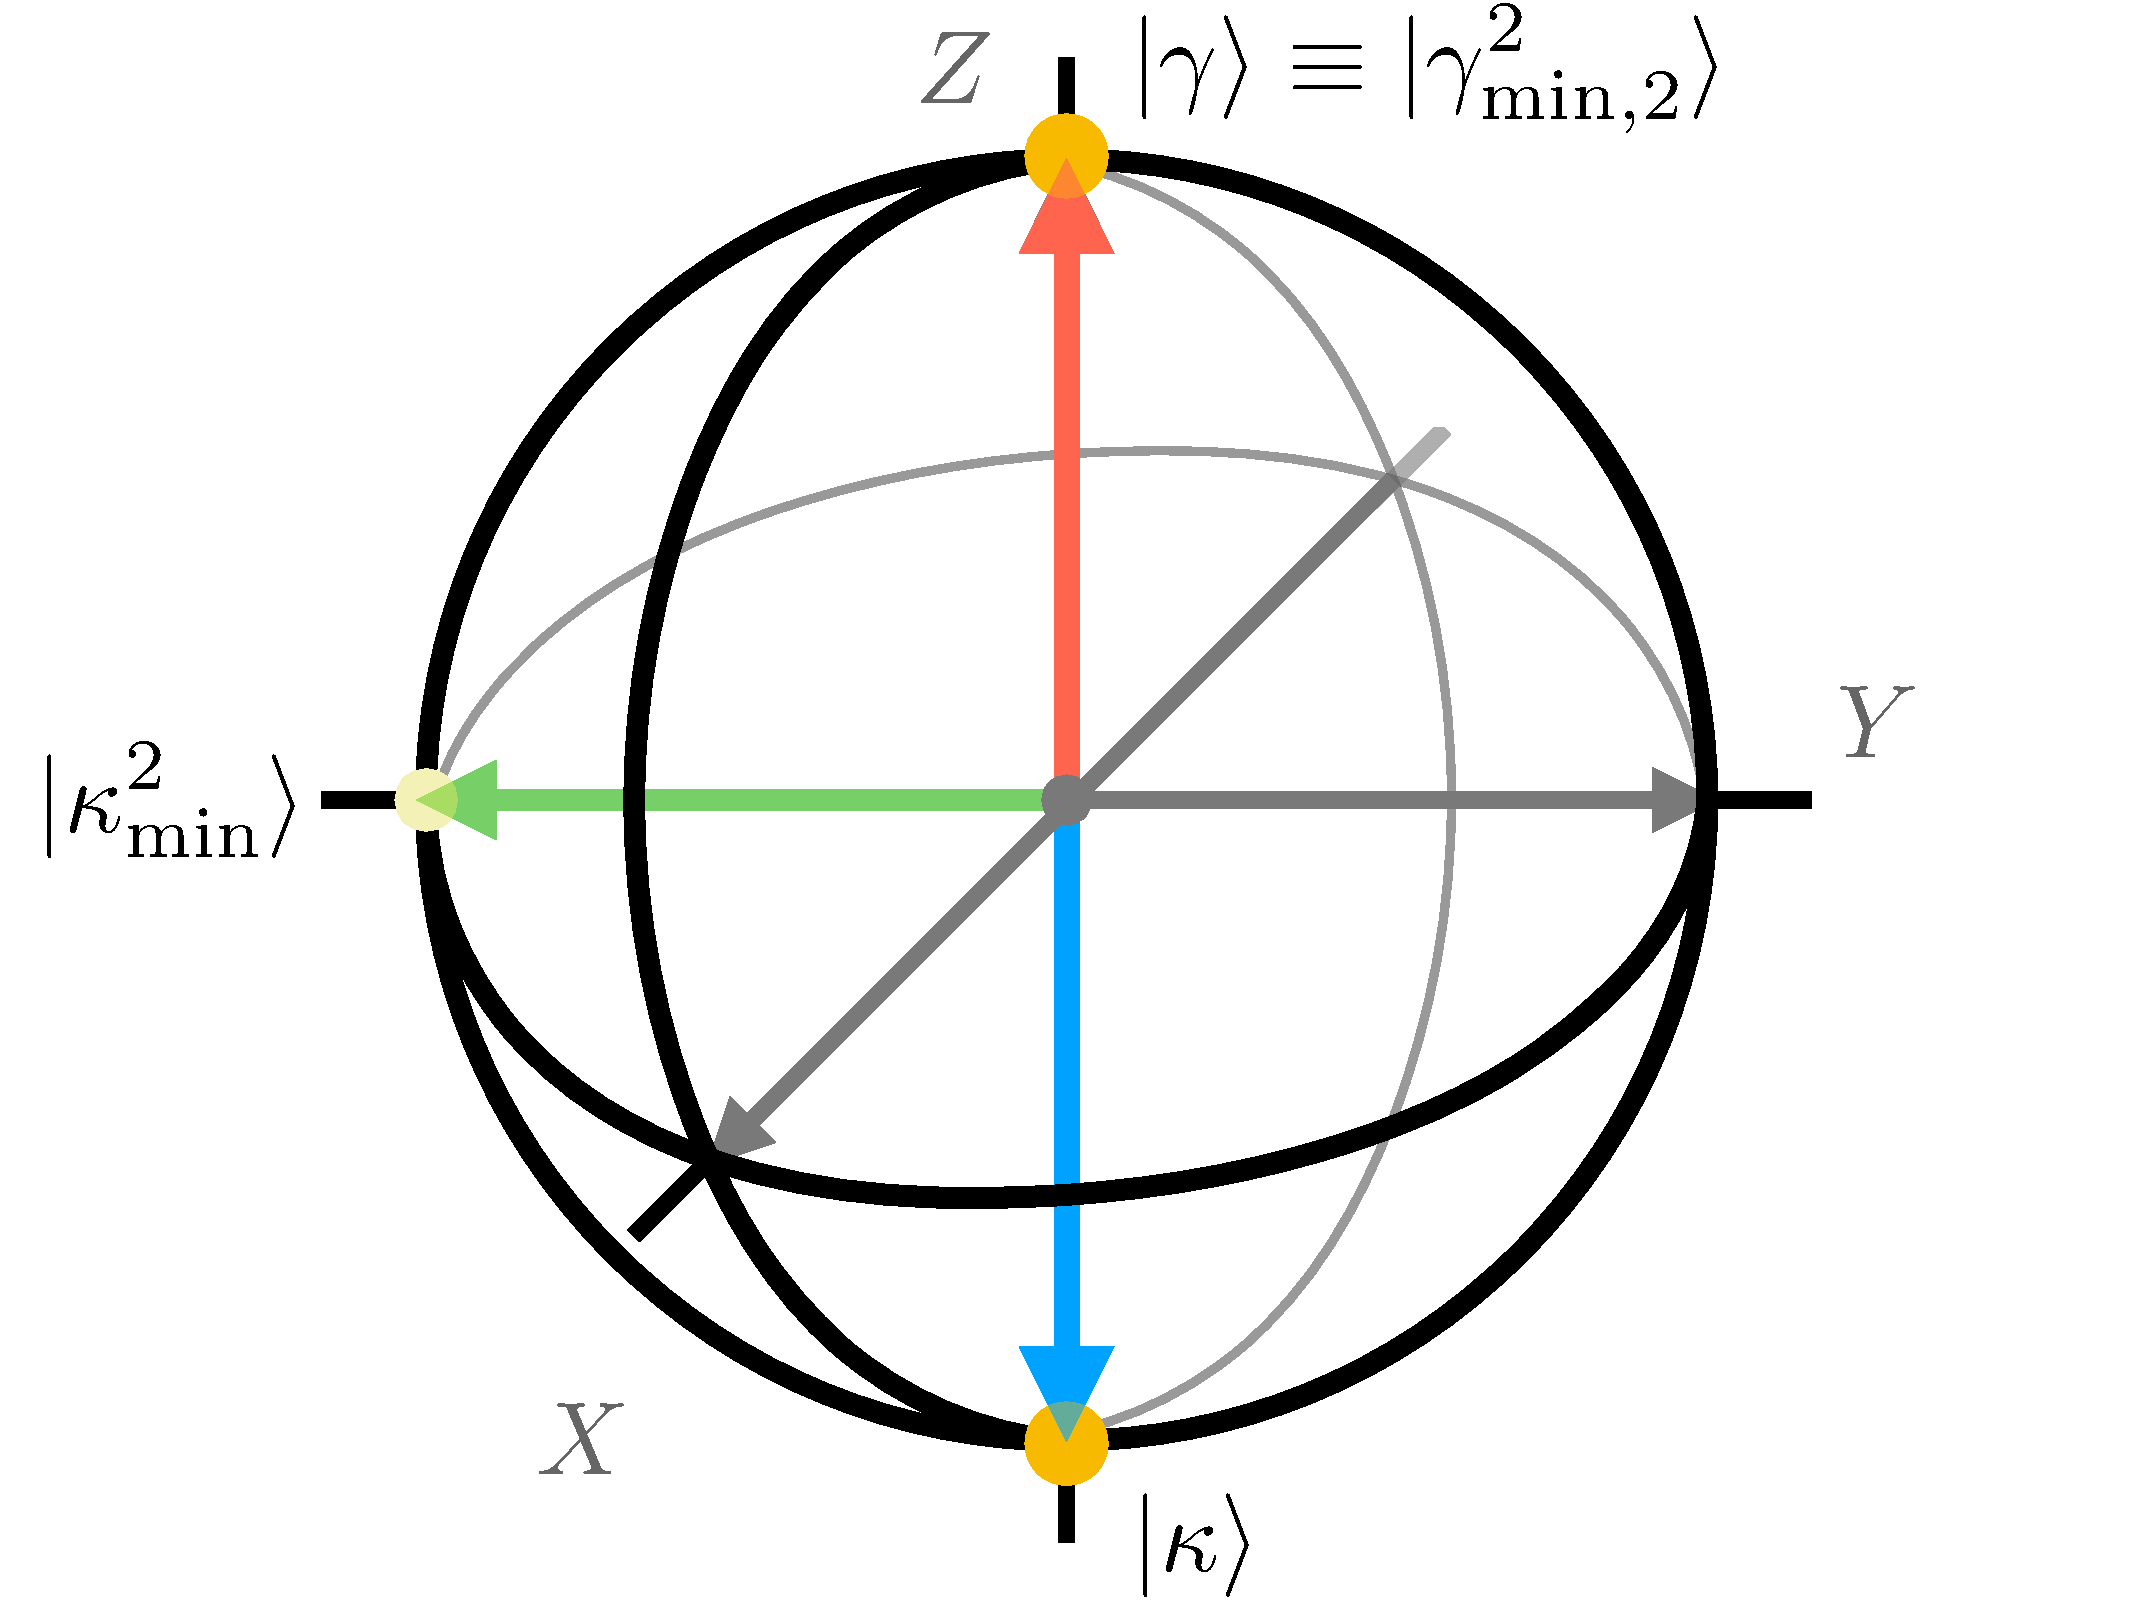
\includegraphics[width=.4\paperwidth]{Figures/NJL1-model-solving/bloch-sphere}
		\end{center}

	\end{multicols}

\end{frame}

\begin{frame}{State preparation II}

	\begin{figure}[!p]
		\centering
		\begin{minipage}[c]{.45\linewidth}
			\centering
			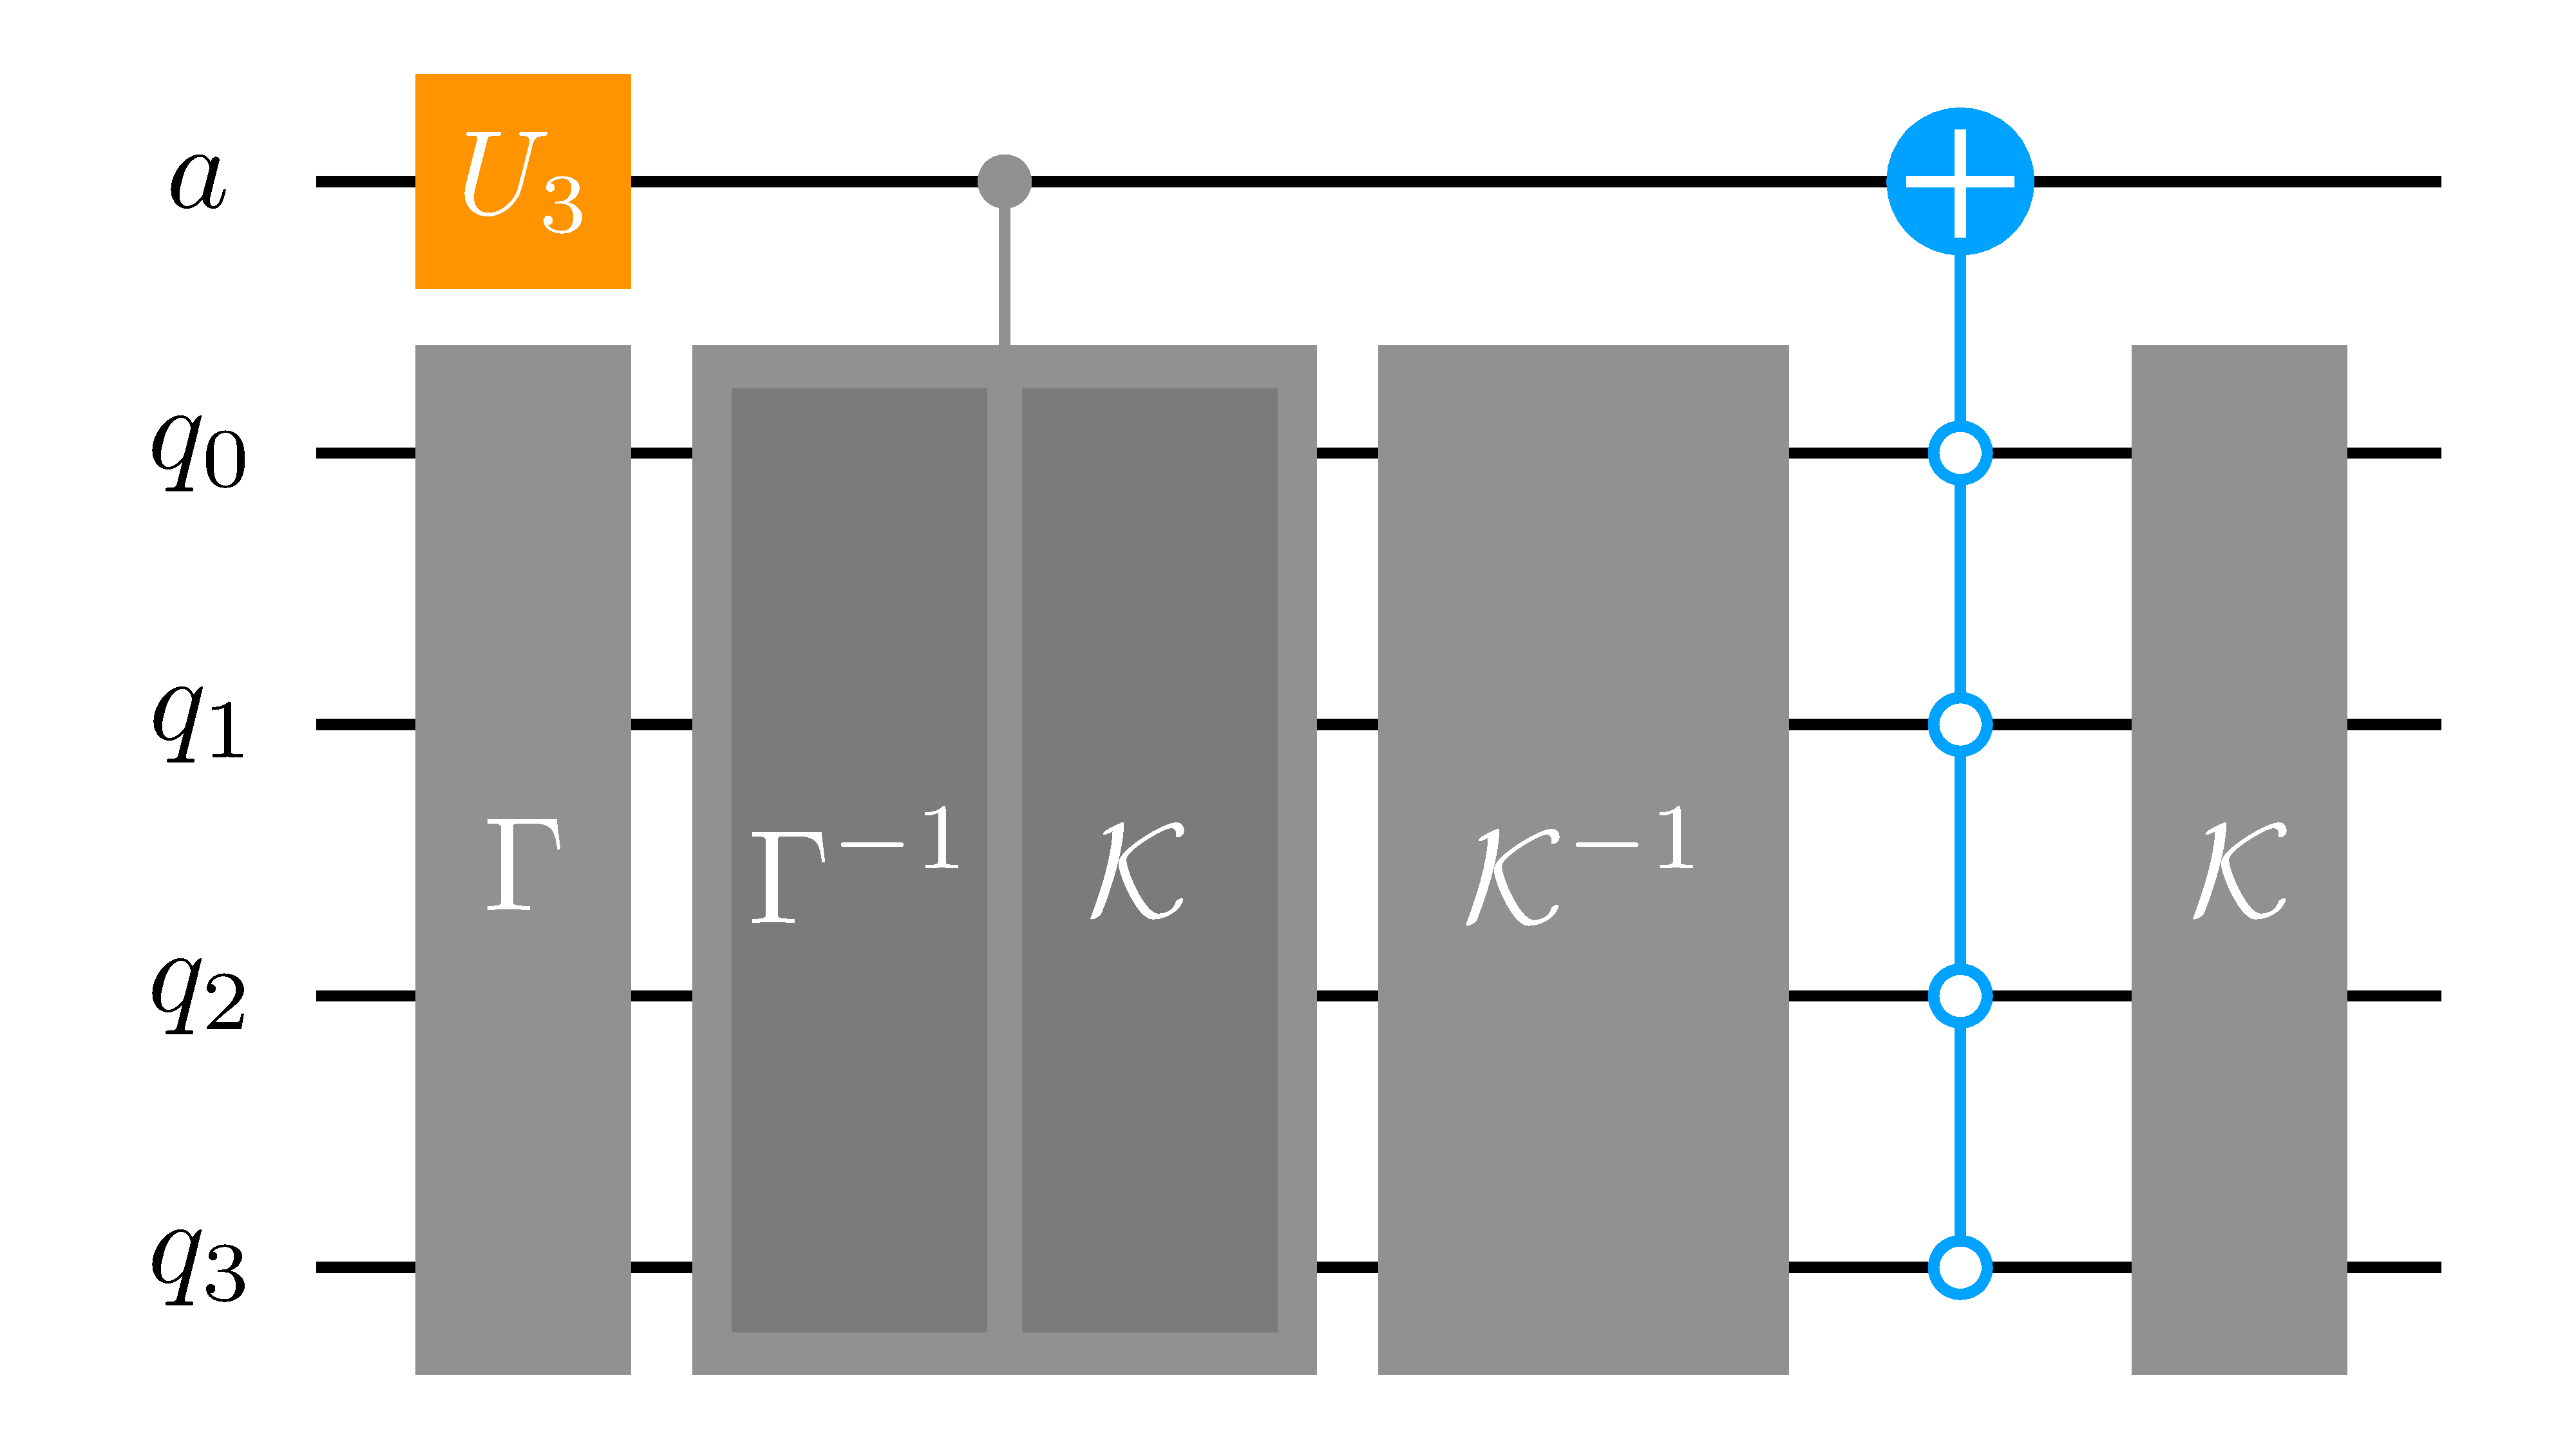
\includegraphics[width=\linewidth]{Figures/NJL1-model-solving/ansatz-implementation-circuit}
		\end{minipage}
		\hspace{.025\linewidth}
		\begin{minipage}[c]{.45\linewidth}
			\centering
			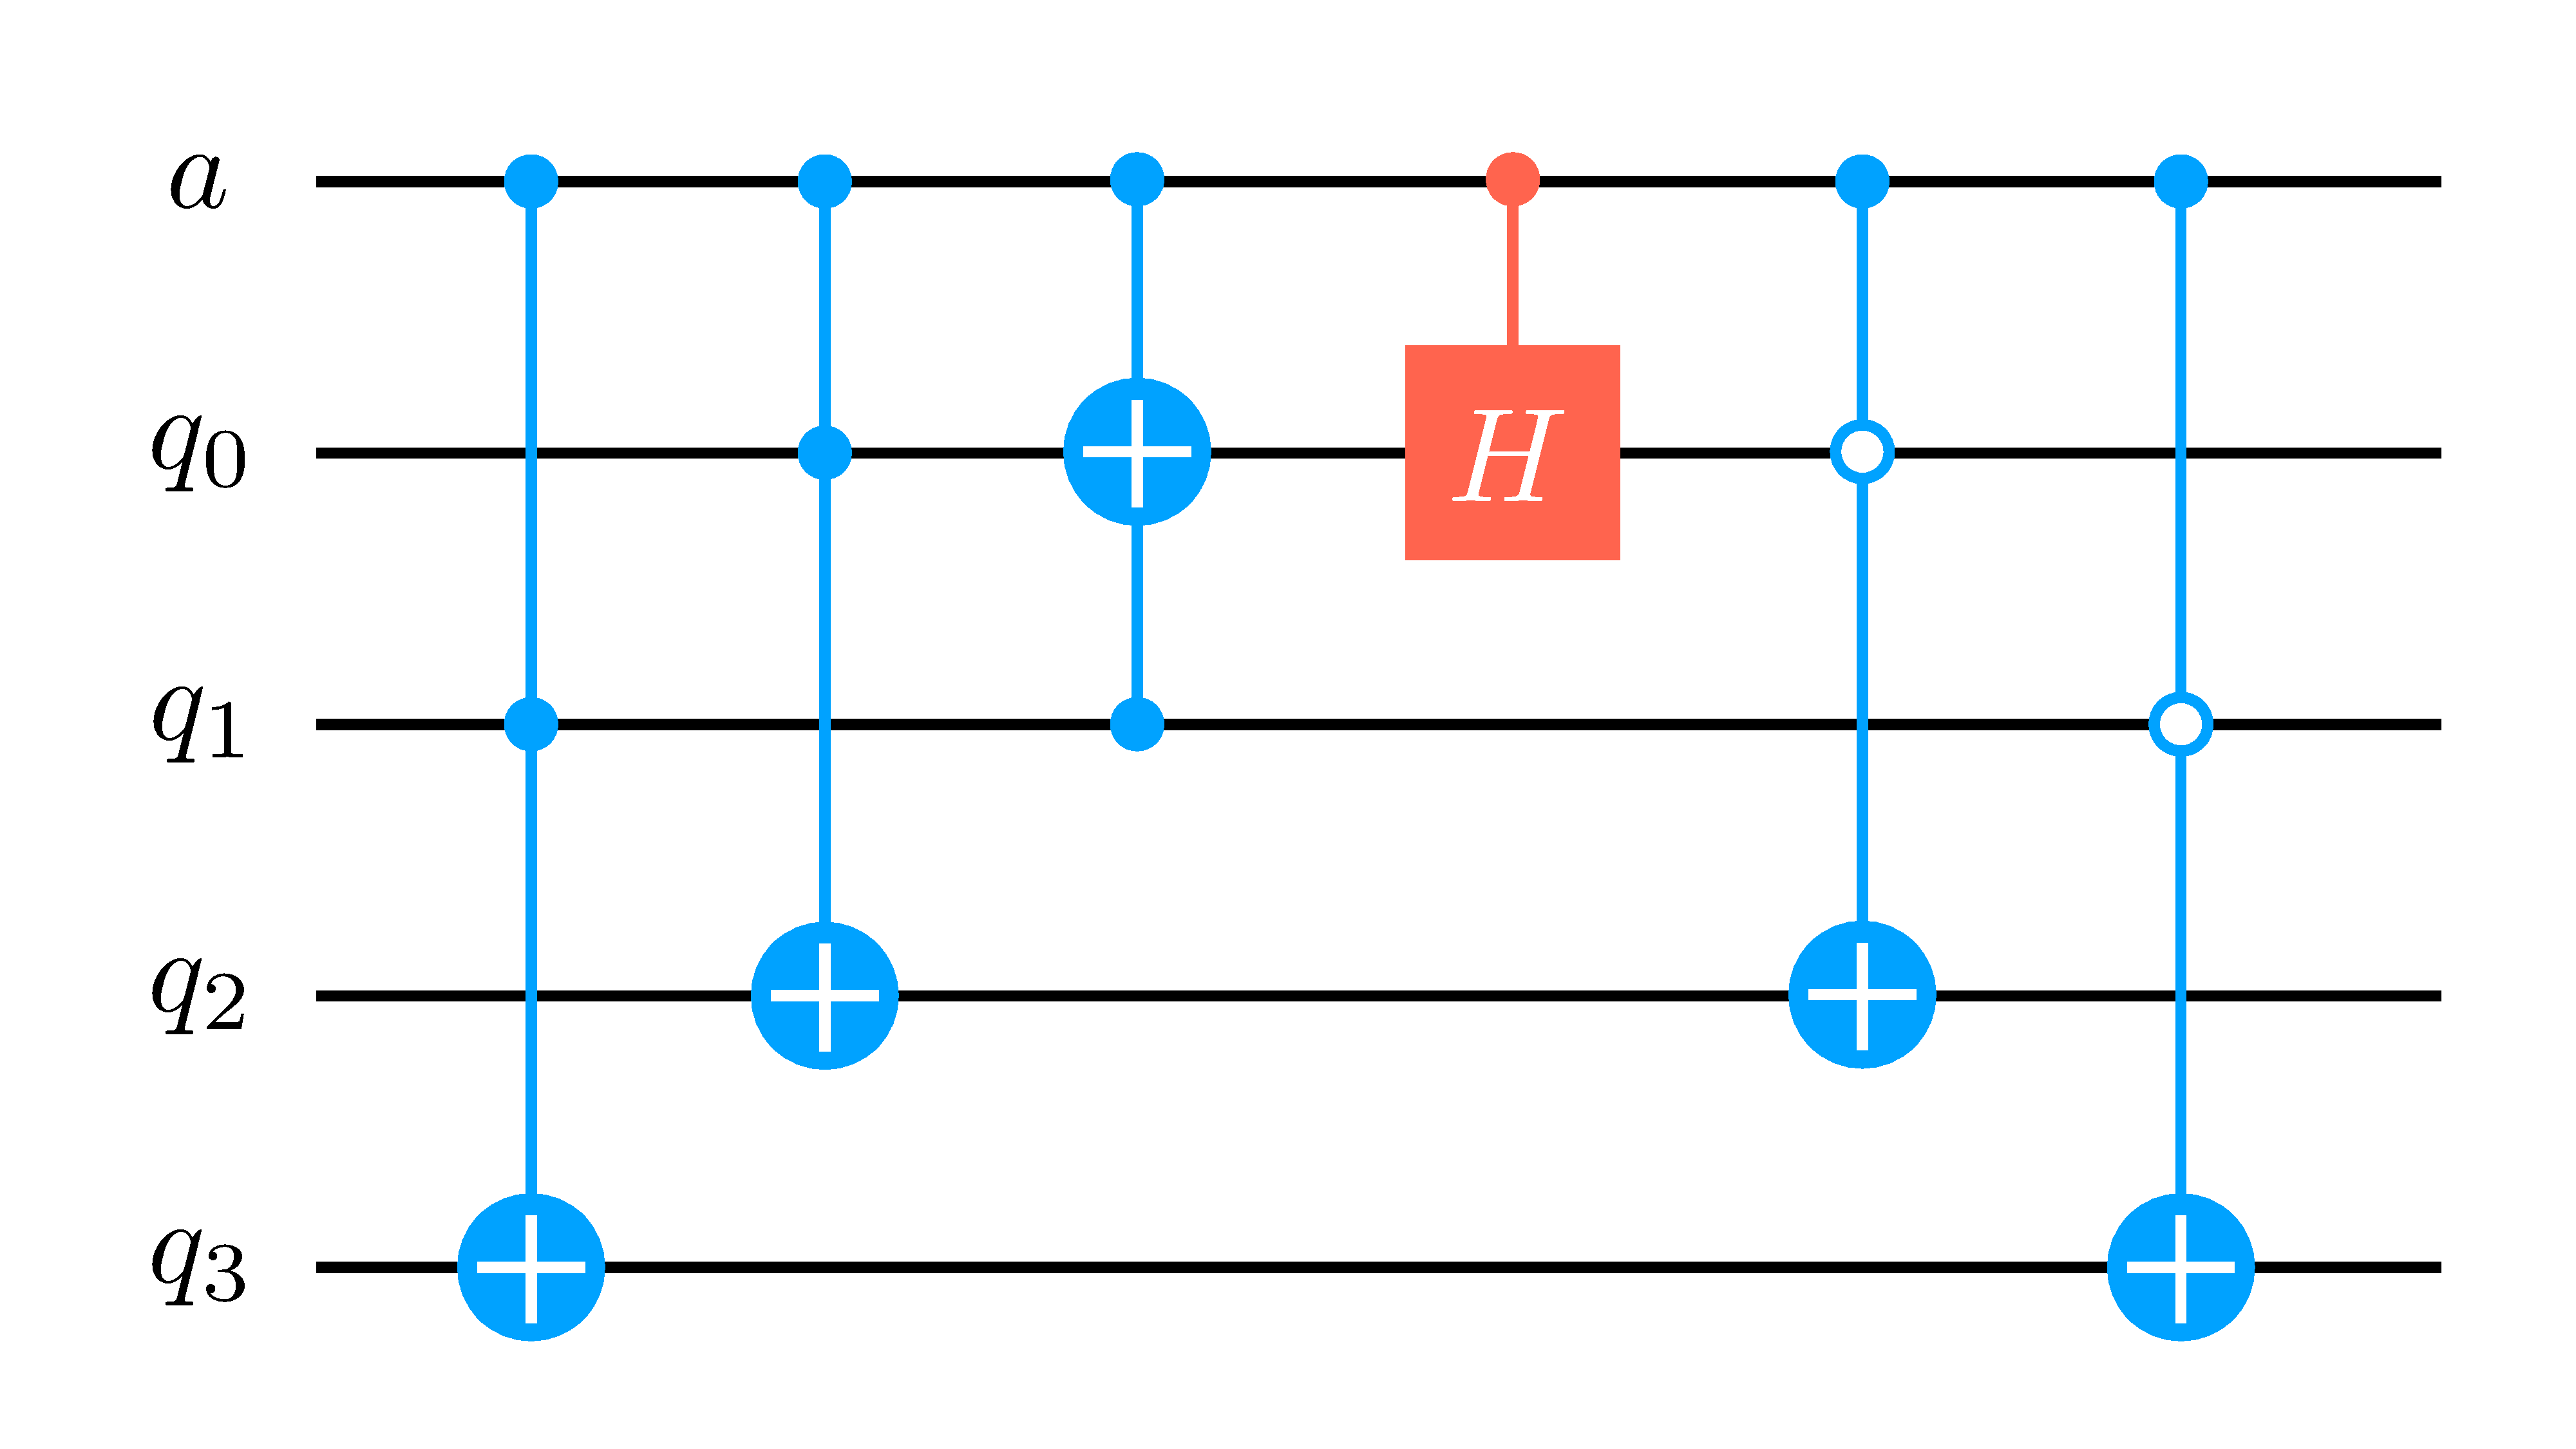
\includegraphics[width=\linewidth]{Figures/NJL1-model-solving/ansatz-implementation-controlled-gammakappa}
		\end{minipage}
		\caption{(Left) Quantum circuit to map the ancilla qubit onto the target qubit Hilbert space in our system. (Right) Simplified controlled $\mathcal{K}\Gamma^{-1}$ gate.}
	\end{figure}

\end{frame}

%% ----------------------------------------------------------------------------

\section{Algorithmic solution}

\begin{frame}{Variational quantum eigensolver algorithm}

	\begin{center}
		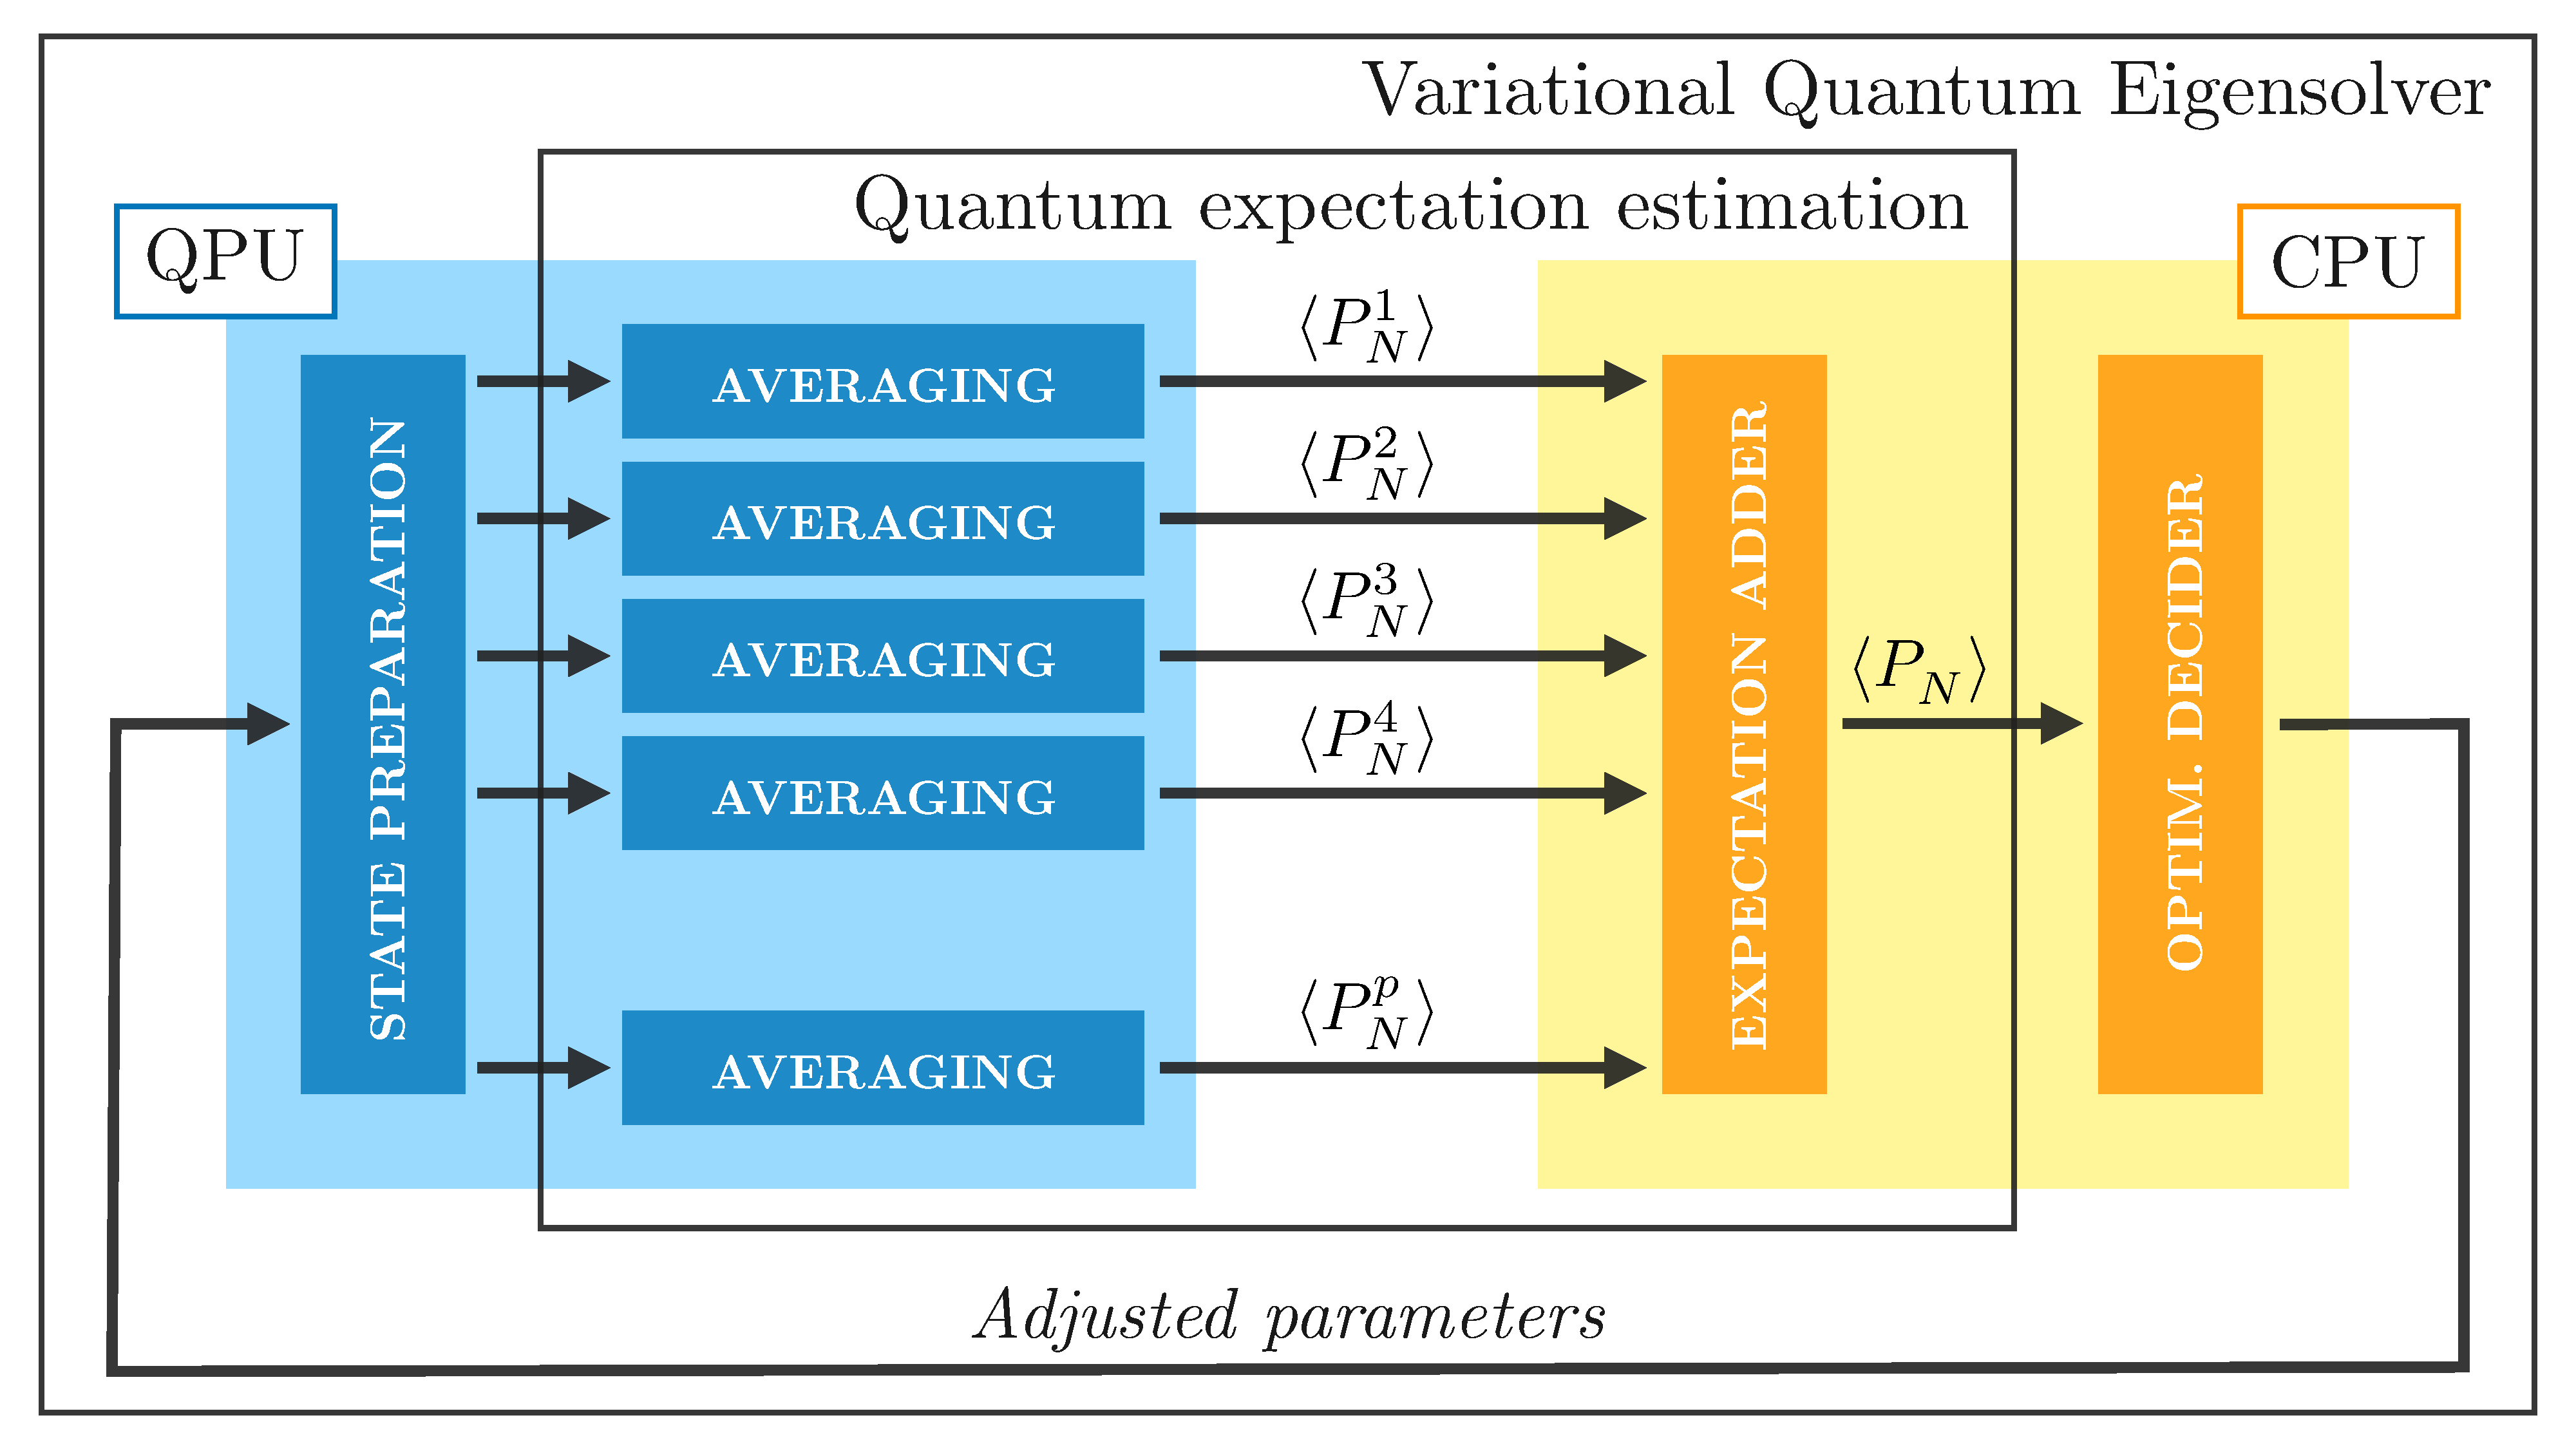
\includegraphics[width=.7\paperwidth]{Figures/NJL1-model-solving/VQE}
	\end{center}

\end{frame}

%% ----------------------------------------------------------------------------

\begin{frame}{Optimal sampling regression algorithm}

	\begin{center}
		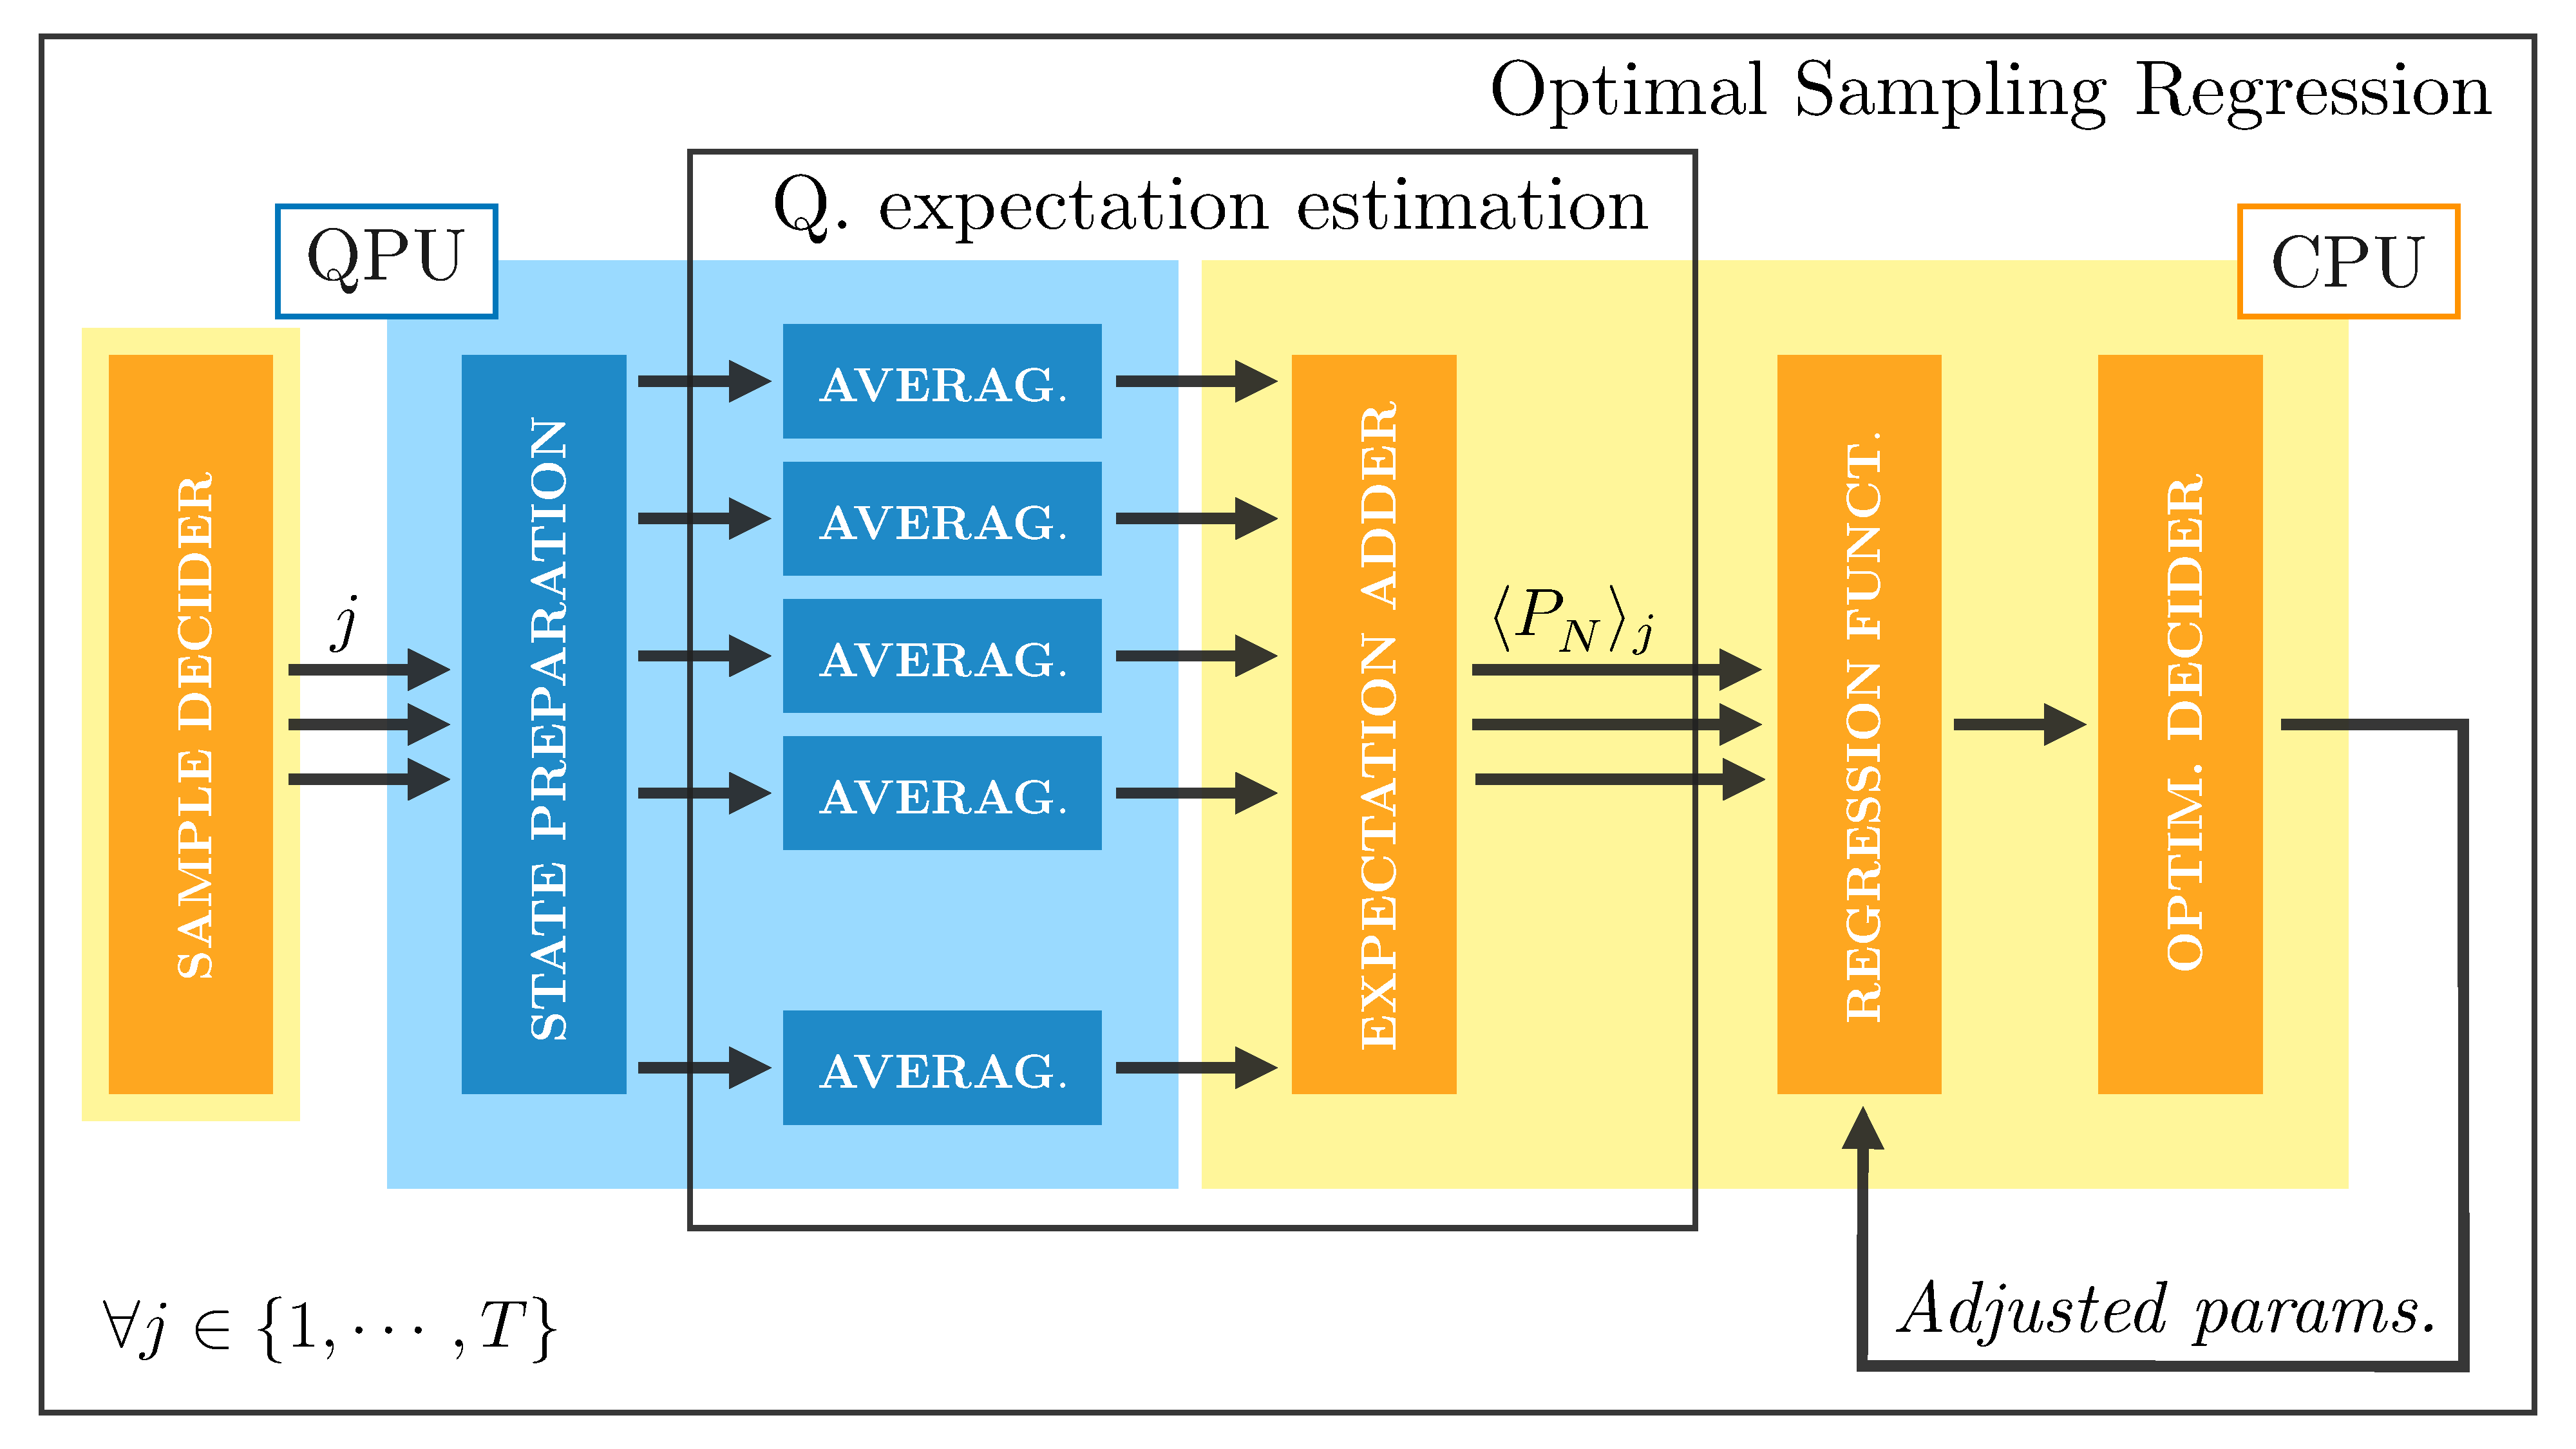
\includegraphics[width=.7\paperwidth]{Figures/NJL1-model-solving/OSR}
	\end{center}

\end{frame}

%% ----------------------------------------------------------------------------

\begin{frame}{Algorithm comparison}

\begin{figure}[!tbp]
	\centering
	\begin{minipage}[c]{.40\linewidth}
		\centering
		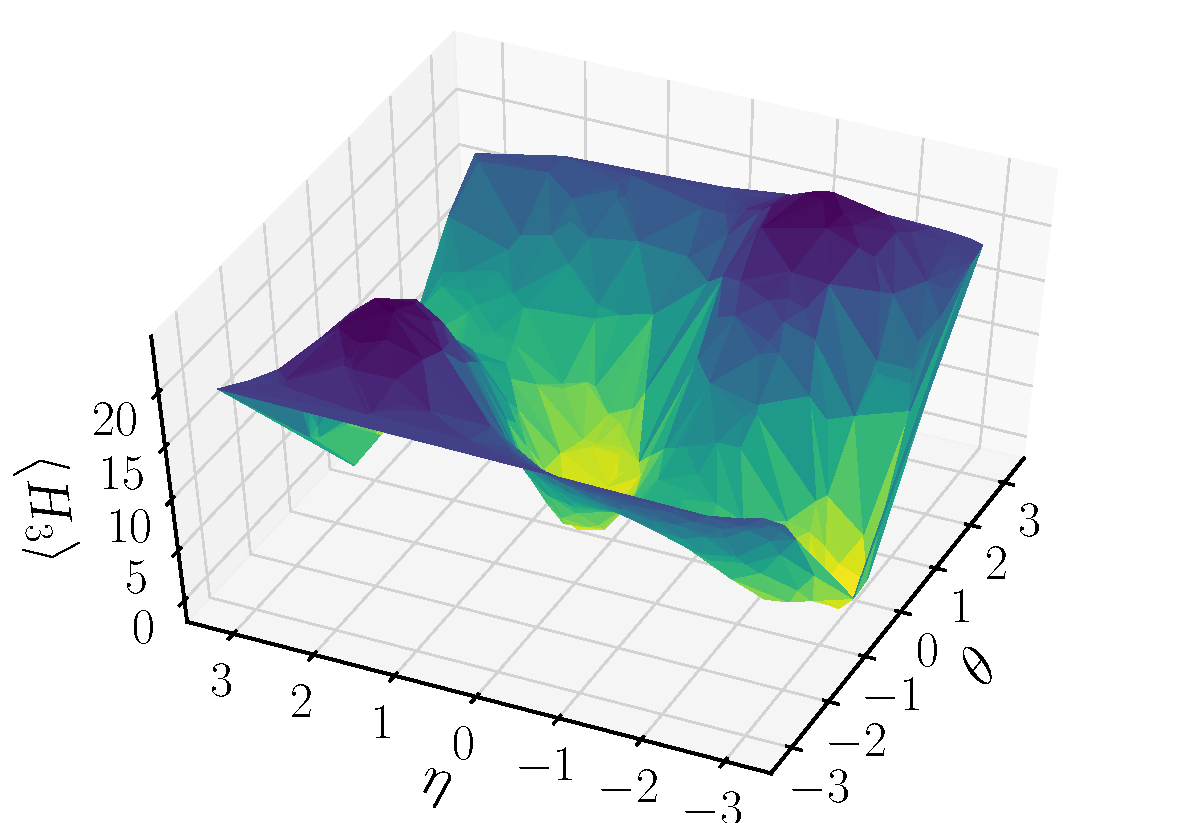
\includegraphics[width=\linewidth]{Figures/NJL1-model-solving/deuteron-VQE}
	\end{minipage}
	\hspace{.025\linewidth}
	\begin{minipage}[c]{.40\linewidth}
		\centering
		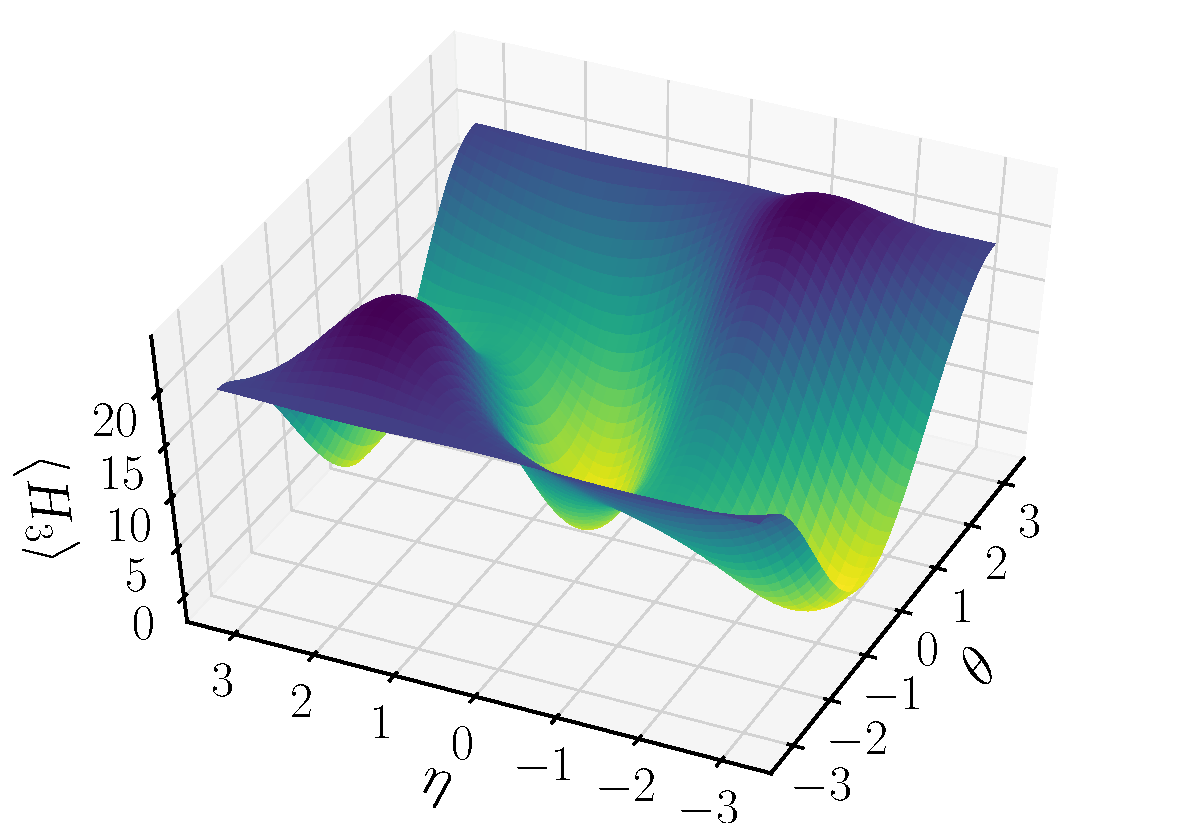
\includegraphics[width=\linewidth]{Figures/NJL1-model-solving/deuteron-OSR}
	\end{minipage}
	\caption{Comparison between the VQE and OSR algorithms, when reproducing an external model with two parameters. (Left) Triangulation of the expectation value function from raw samples. (Right) Approximate function obtained through the Optimal Sampling Regression method with $S_q=S_{\text{max}}=2 ~\forall q$.}
\end{figure}

\vspace{-1em}

\begin{table}[!bp]
	\centering
	% \caption{Comparison between results using the VQE and OSR algorithms.}
	\begin{tabular}{ c c c c c }
		\hline
		% \rule{0pt}{14pt}
		$N_\text{params}$ & VQE samples & OSR samples &
		VQE error & OSR error \\
		\hline
		\hline
		% \rule{0pt}{14pt}
		$1$ & $24$ & $3$ & $3.5\%$ & $1.0\%$ \\
		\hline
		$2$ & $153$ & $25$ & $0.3\%$ & $0.2\%$ \\
		\hline
	\end{tabular}
\end{table}

\end{frame}

%% ----------------------------------------------------------------------------

\subsection{Ground state energy}

\begin{frame}[allowframebreaks]{Ground state energy}

	At last, we have everything that we need to solve for the ground state energy of our system using a quantum computer. For simplicity, we will do so first through a \textbf{quantum simulator}.

	\begin{center}
		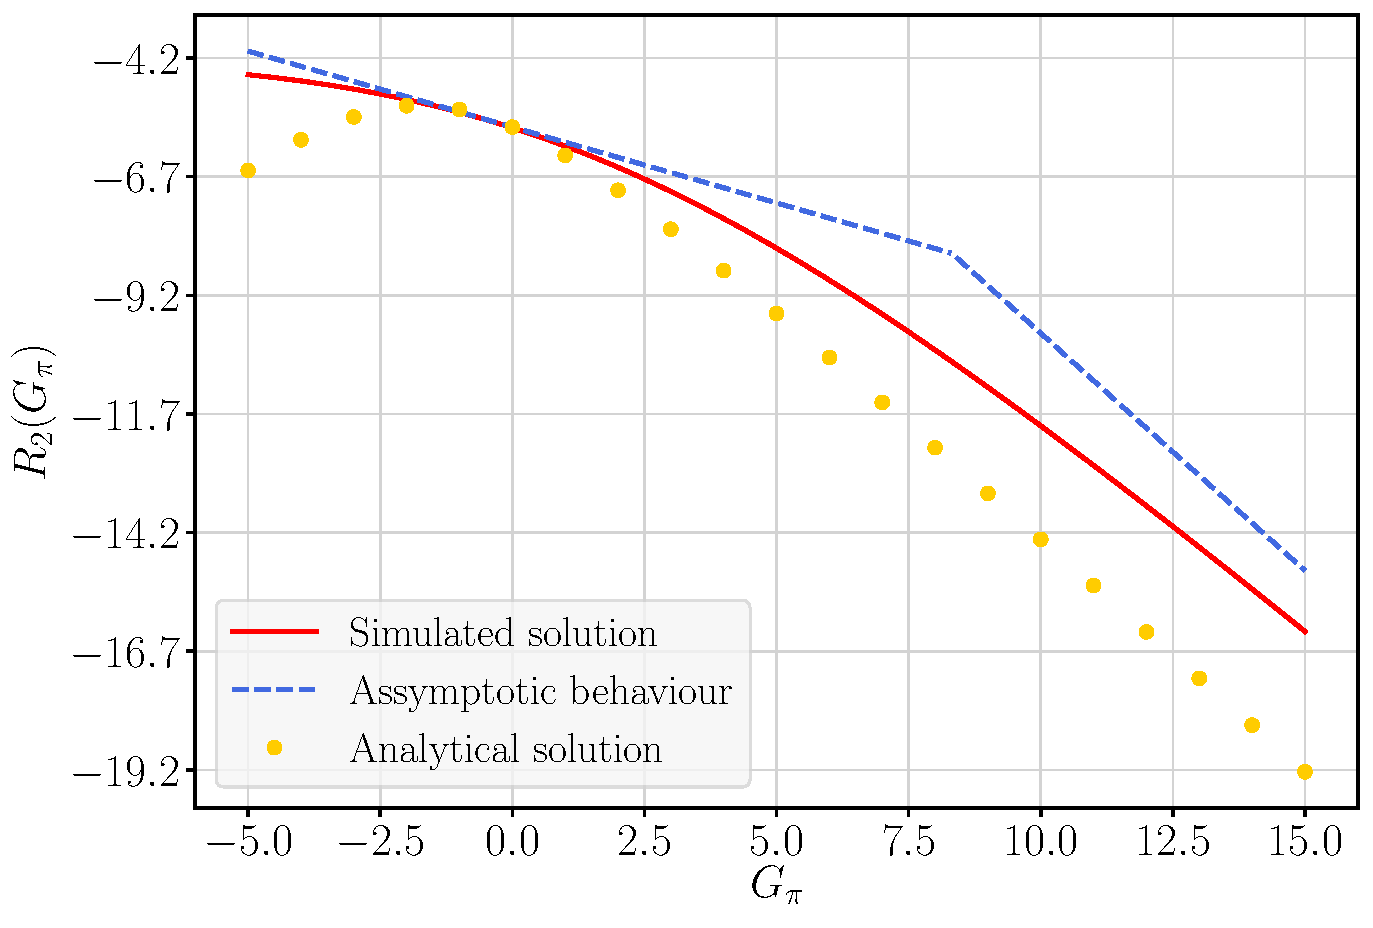
\includegraphics[width=.45\paperwidth]{Figures/NJL1-model-solving/G2}
	\end{center}
	\vspace{-2em}

\break

	\begin{figure}[!p]
		\centering
		\begin{minipage}[c]{.4\linewidth}
			\centering
			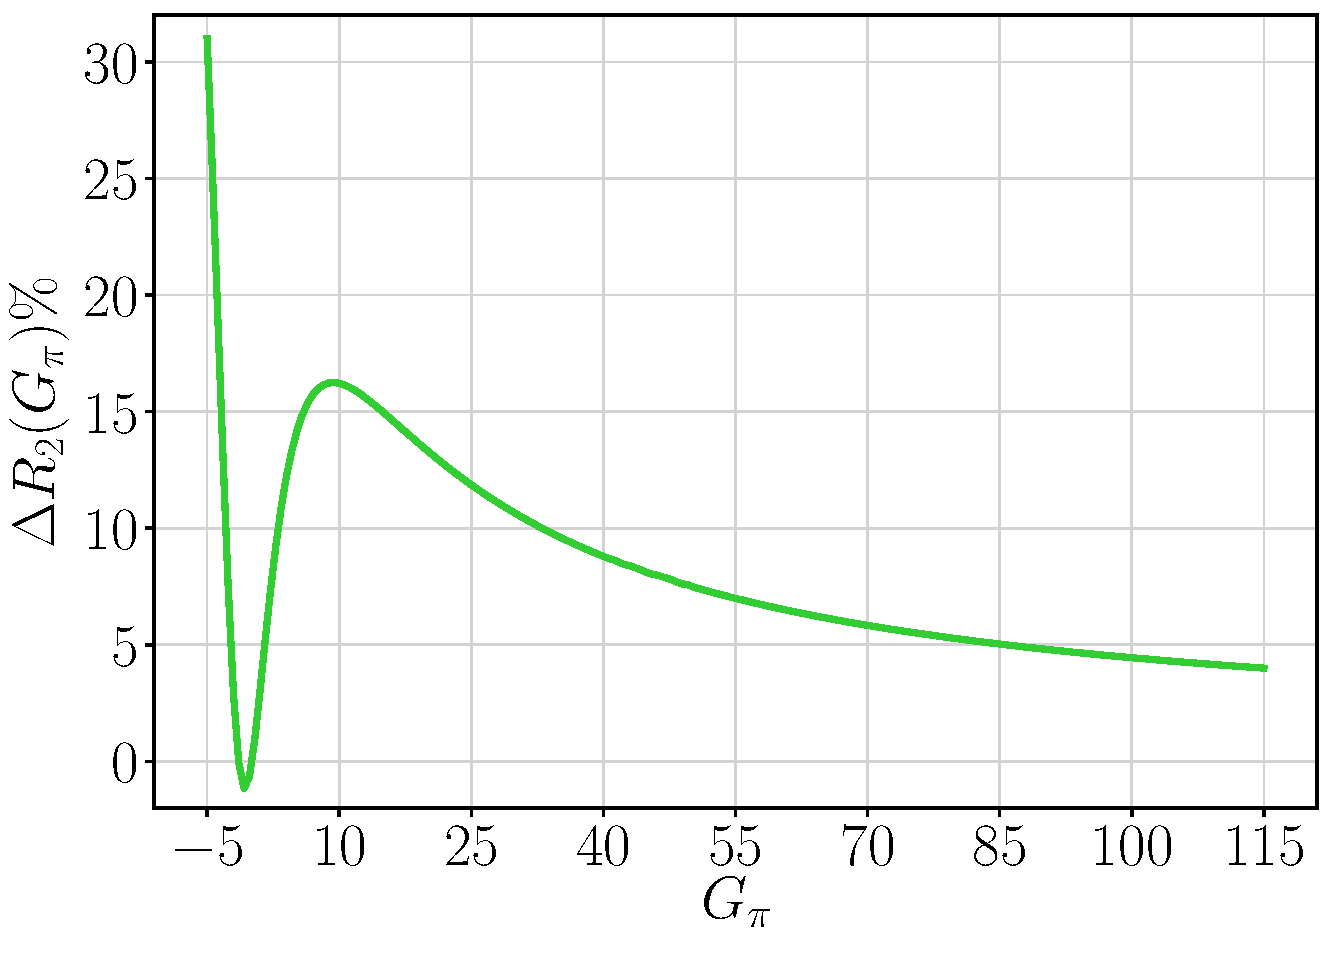
\includegraphics[width=.8\linewidth]{Figures/NJL1-model-solving/G2-err}
		\end{minipage}
		\hspace{.025\linewidth}
		\begin{minipage}[c]{.4\linewidth}
			\centering
			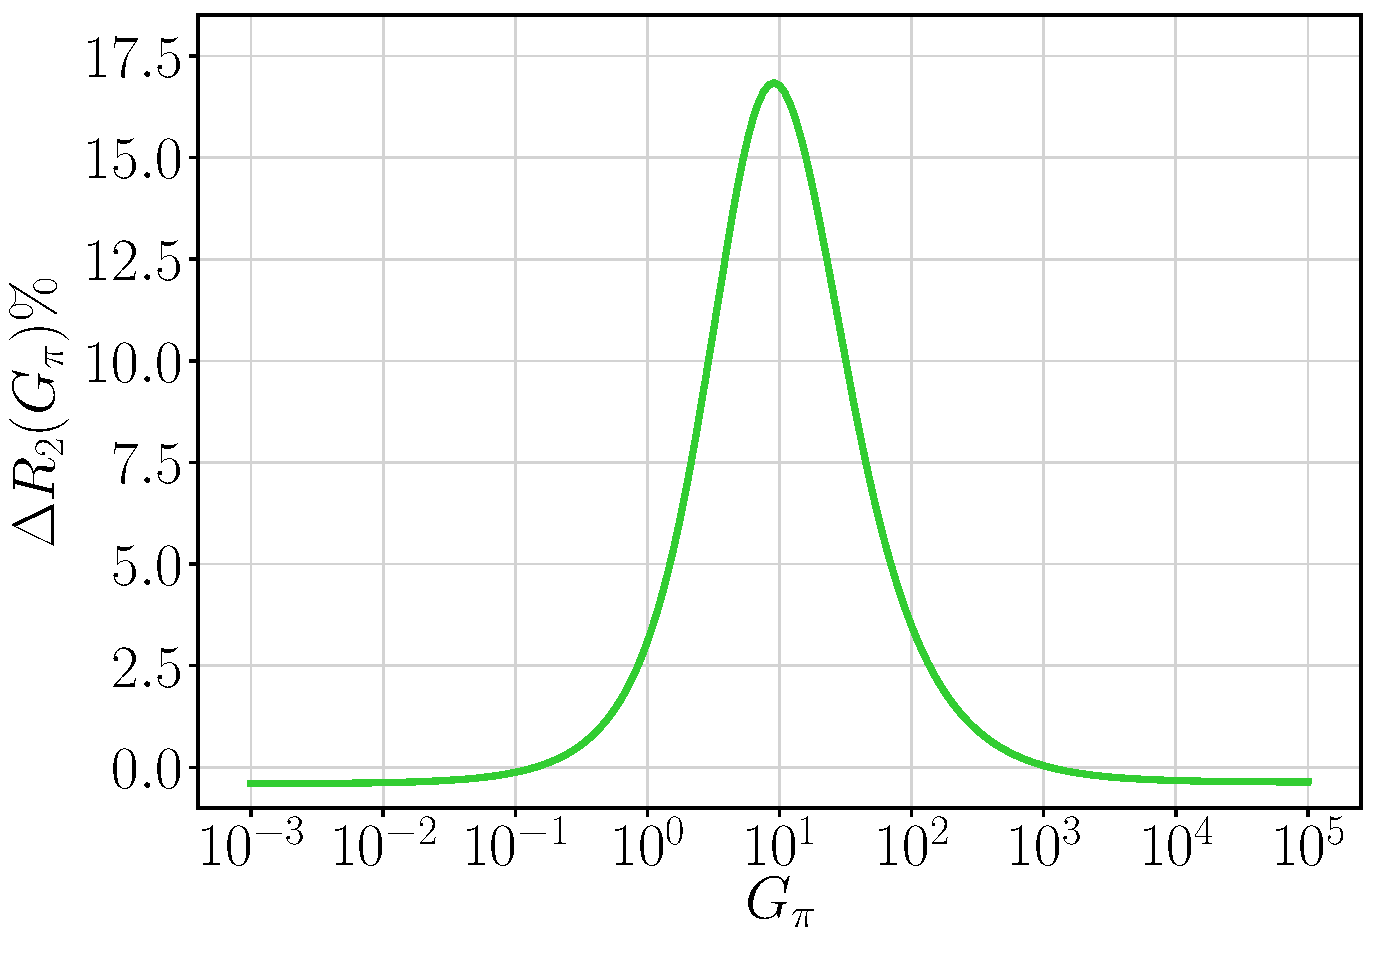
\includegraphics[width=.8\linewidth]{Figures/NJL1-model-solving/G2-logerr}
		\end{minipage} \\[-1em]
		\begin{center}
			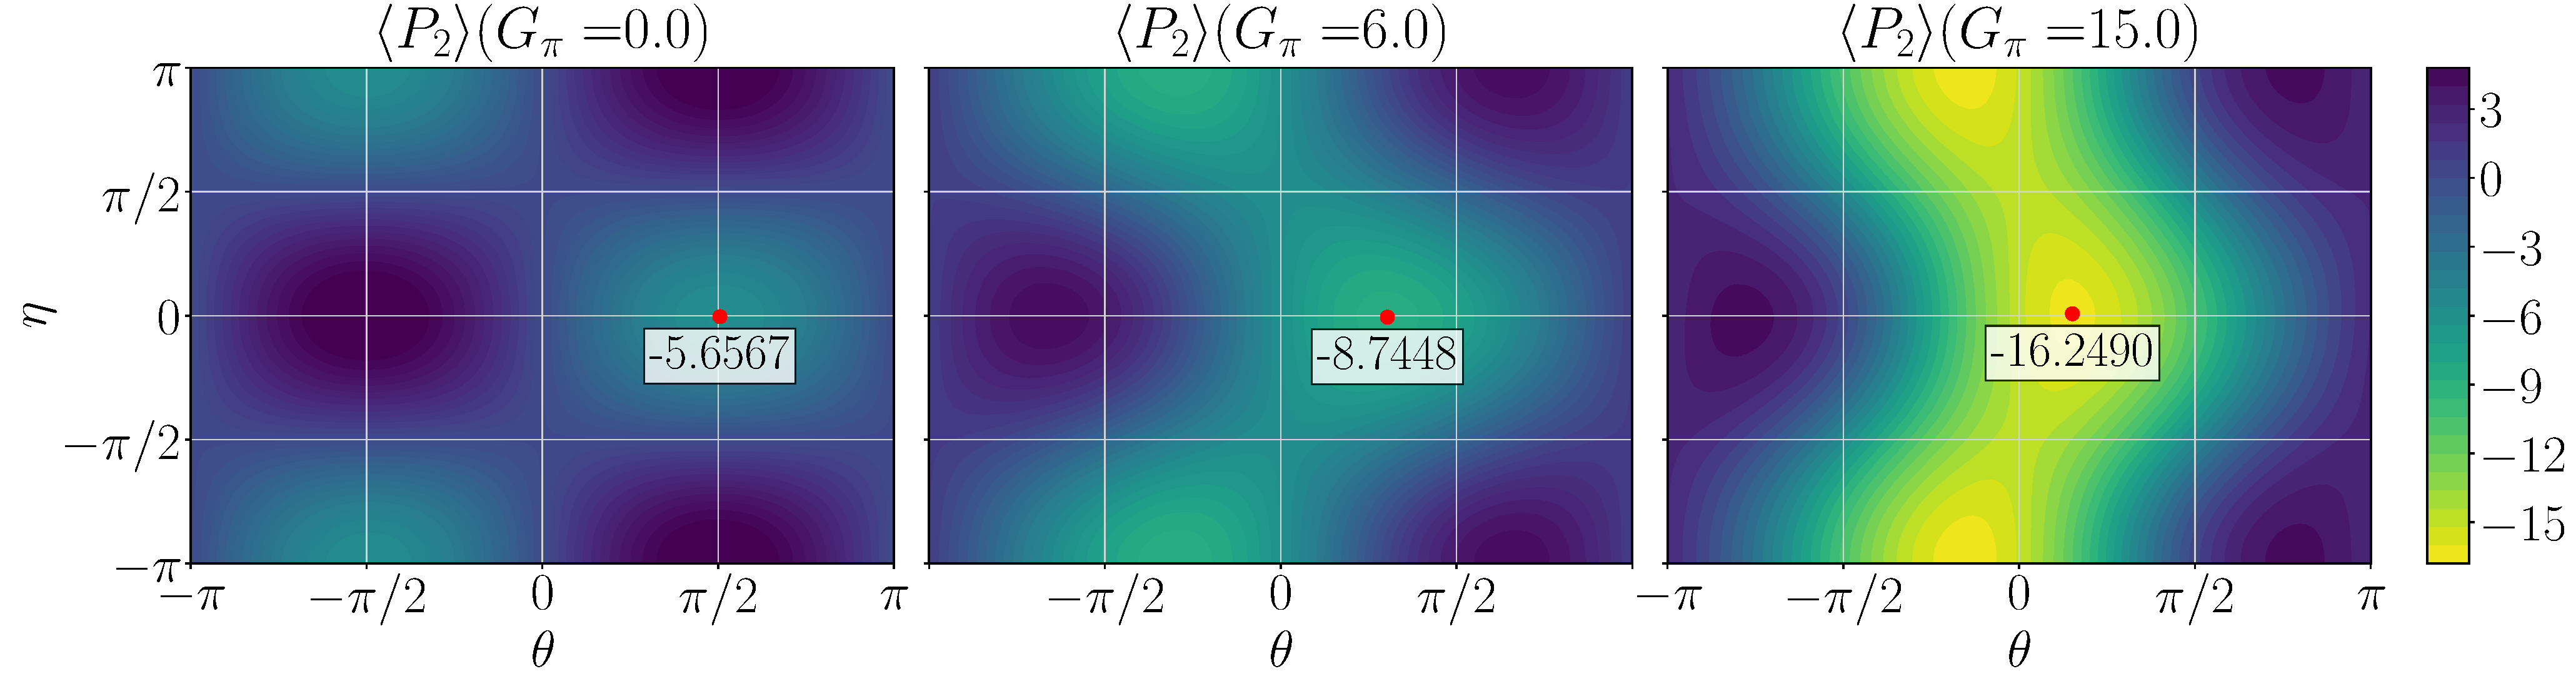
\includegraphics[width=.7\paperwidth]{Figures/NJL1-model-solving/P2-tri-contour}
		\end{center}
		% \caption{Percentual error of the ground state energy results obtained from our quantum simulation with respect to the analytical solution and for different values of the coupling constant. (Left) Linear scale. (Right) Logarithmic scale.}
	\end{figure}
	\vspace{-2em}

\end{frame}


%% ----------------------------------------------------------------------------
%% BACK-MATTER
%% ----------------------------------------------------------------------------

% \section{Bibliography}
% %	\begin{frame}[allowframebreaks]{Bibliography}
% \begin{frame}{Bibliography}
%
% 	\begin{thebibliography}{9}
% 		\setbeamertemplate{bibliography item}[online]
% 	\bibitem{hayden} \textbf{Hayden, P.} \emph{Quantum Computational Universe}
% 		\setbeamertemplate{bibliography item}[book]
% 	\bibitem{susskind_book} \textbf{Susskind, L. \& Friedman A.} \emph{Quantum Mechanics: The Theoretical Minimum}
% 		\setbeamertemplate{bibliography item}[book]
% 	\bibitem{nielsen} \textbf{Nielsen M.A. \& Chuang I.L.} \emph{Quantum Computation and Quantum Information}
% 		\setbeamertemplate{bibliography item}[article]
% 	\bibitem{ladd} \textbf{Lykken J.} \emph{Quantum Technologies for Quantum Science}
% 		\setbeamertemplate{bibliography item}[book]
% 	\bibitem{mermin} \textbf{Mermin N.D.} \emph{Quantum Computer Science: An Introduction}
% 		\setbeamertemplate{bibliography item}[article]
% 	\bibitem{ladd} \textbf{Ladd T.D. (et al.)} \emph{Quantum Computing}
%
% 	\end{thebibliography}
%
% 	\vspace{20pt}
% 	\begin{small}
% 	\begin{center}{
% 	\color{gray}
% 		\emph{"The only thing demonstrated by an impossibility proof is a lack of imagination."} \\
% 		\textbf{– John Stewart Bell –} }
% 	\end{center}
% 	\end{small}
% \end{frame}

%% ----------------------------------------------------------------------------

\FinalFrame

%% ----------------------------------------------------------------------------
%% EXTRA CONTENT
%% ----------------------------------------------------------------------------

\begin{frame}{Dirac equation from staggered fermion lattice}

	From the kinetic term of the discretized Hamiltonian, we can now recover the \textbf{masless Dirac equation} in the continuum limit; which serves as proof of correctness:

	\begin{gather*}
	  \dot{\phi}(n) = i\com{H_{N}^{(K)}}{\phi(n)} = \frac{\phi(n+1)-\phi(n-1)}{a}
	\end{gather*}

	In terms of the original fields, this is:

	\begin{gather*}
	  \dot{\psi_{+}} = \frac{\Delta \psi_{-}}{\Delta x} \qc
	  \dot{\psi_{-}} = \frac{\Delta \psi_{+}}{\Delta x}
	\end{gather*}

	Lastly, taking the limit when $a \ra 0$:

	\begin{gather*}
	  \pderivative{t}\psi = \hat{\alpha_1}\pderivative{x}\psi \\
	  \hat{\alpha_1} \defeq \gamma_{0}\gamma_{1} = \gamma^{0}\gamma_{1}
	    = -\gamma^{0}\gamma^{1} = \mqty[0 & 1 \\ 1 & 0]
	\end{gather*}

\end{frame}

%% ----------------------------------------------------------------------------

\begin{frame}[allowframebreaks]{State preparation low level circuits}

	\begin{figure}[!p]
		\centering
		\begin{minipage}[c]{.45\linewidth}
			\centering
			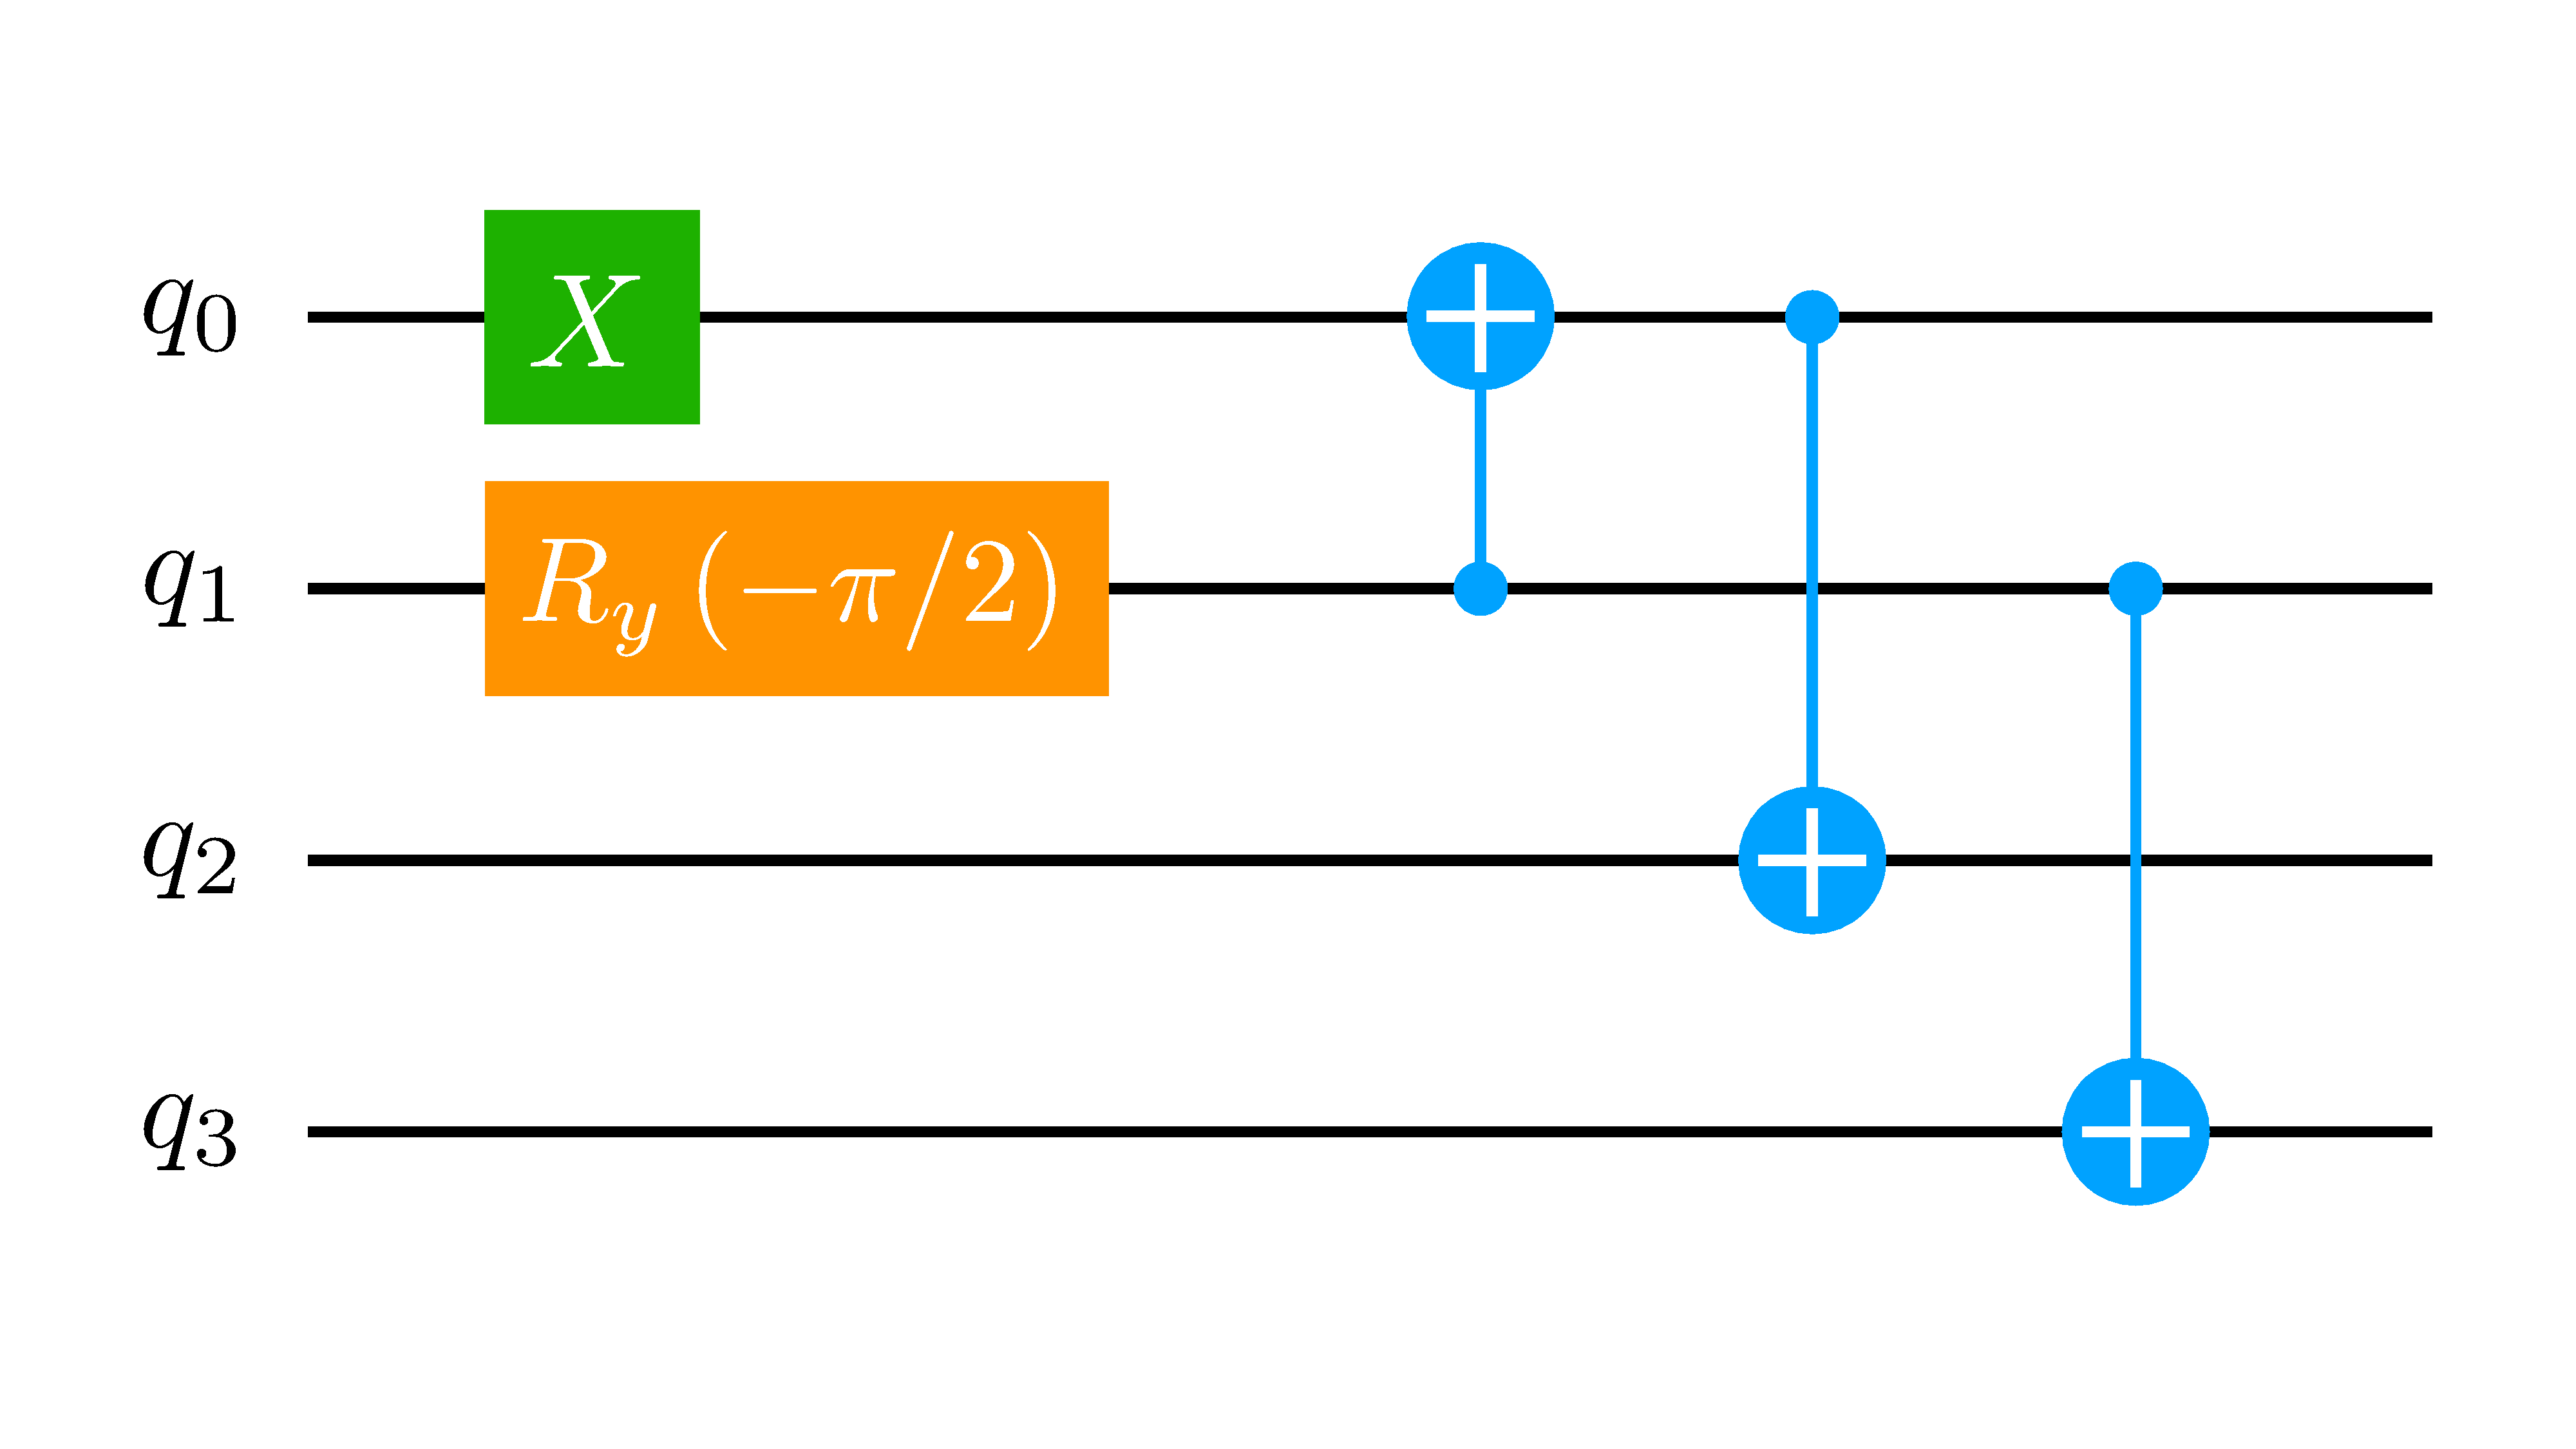
\includegraphics[width=\linewidth]{Figures/NJL1-model-solving/ansatz-implementation-base-state-preparation-gamma}
		\end{minipage}
	  \hspace{.025\linewidth}
		\begin{minipage}[c]{.45\linewidth}
			\centering
			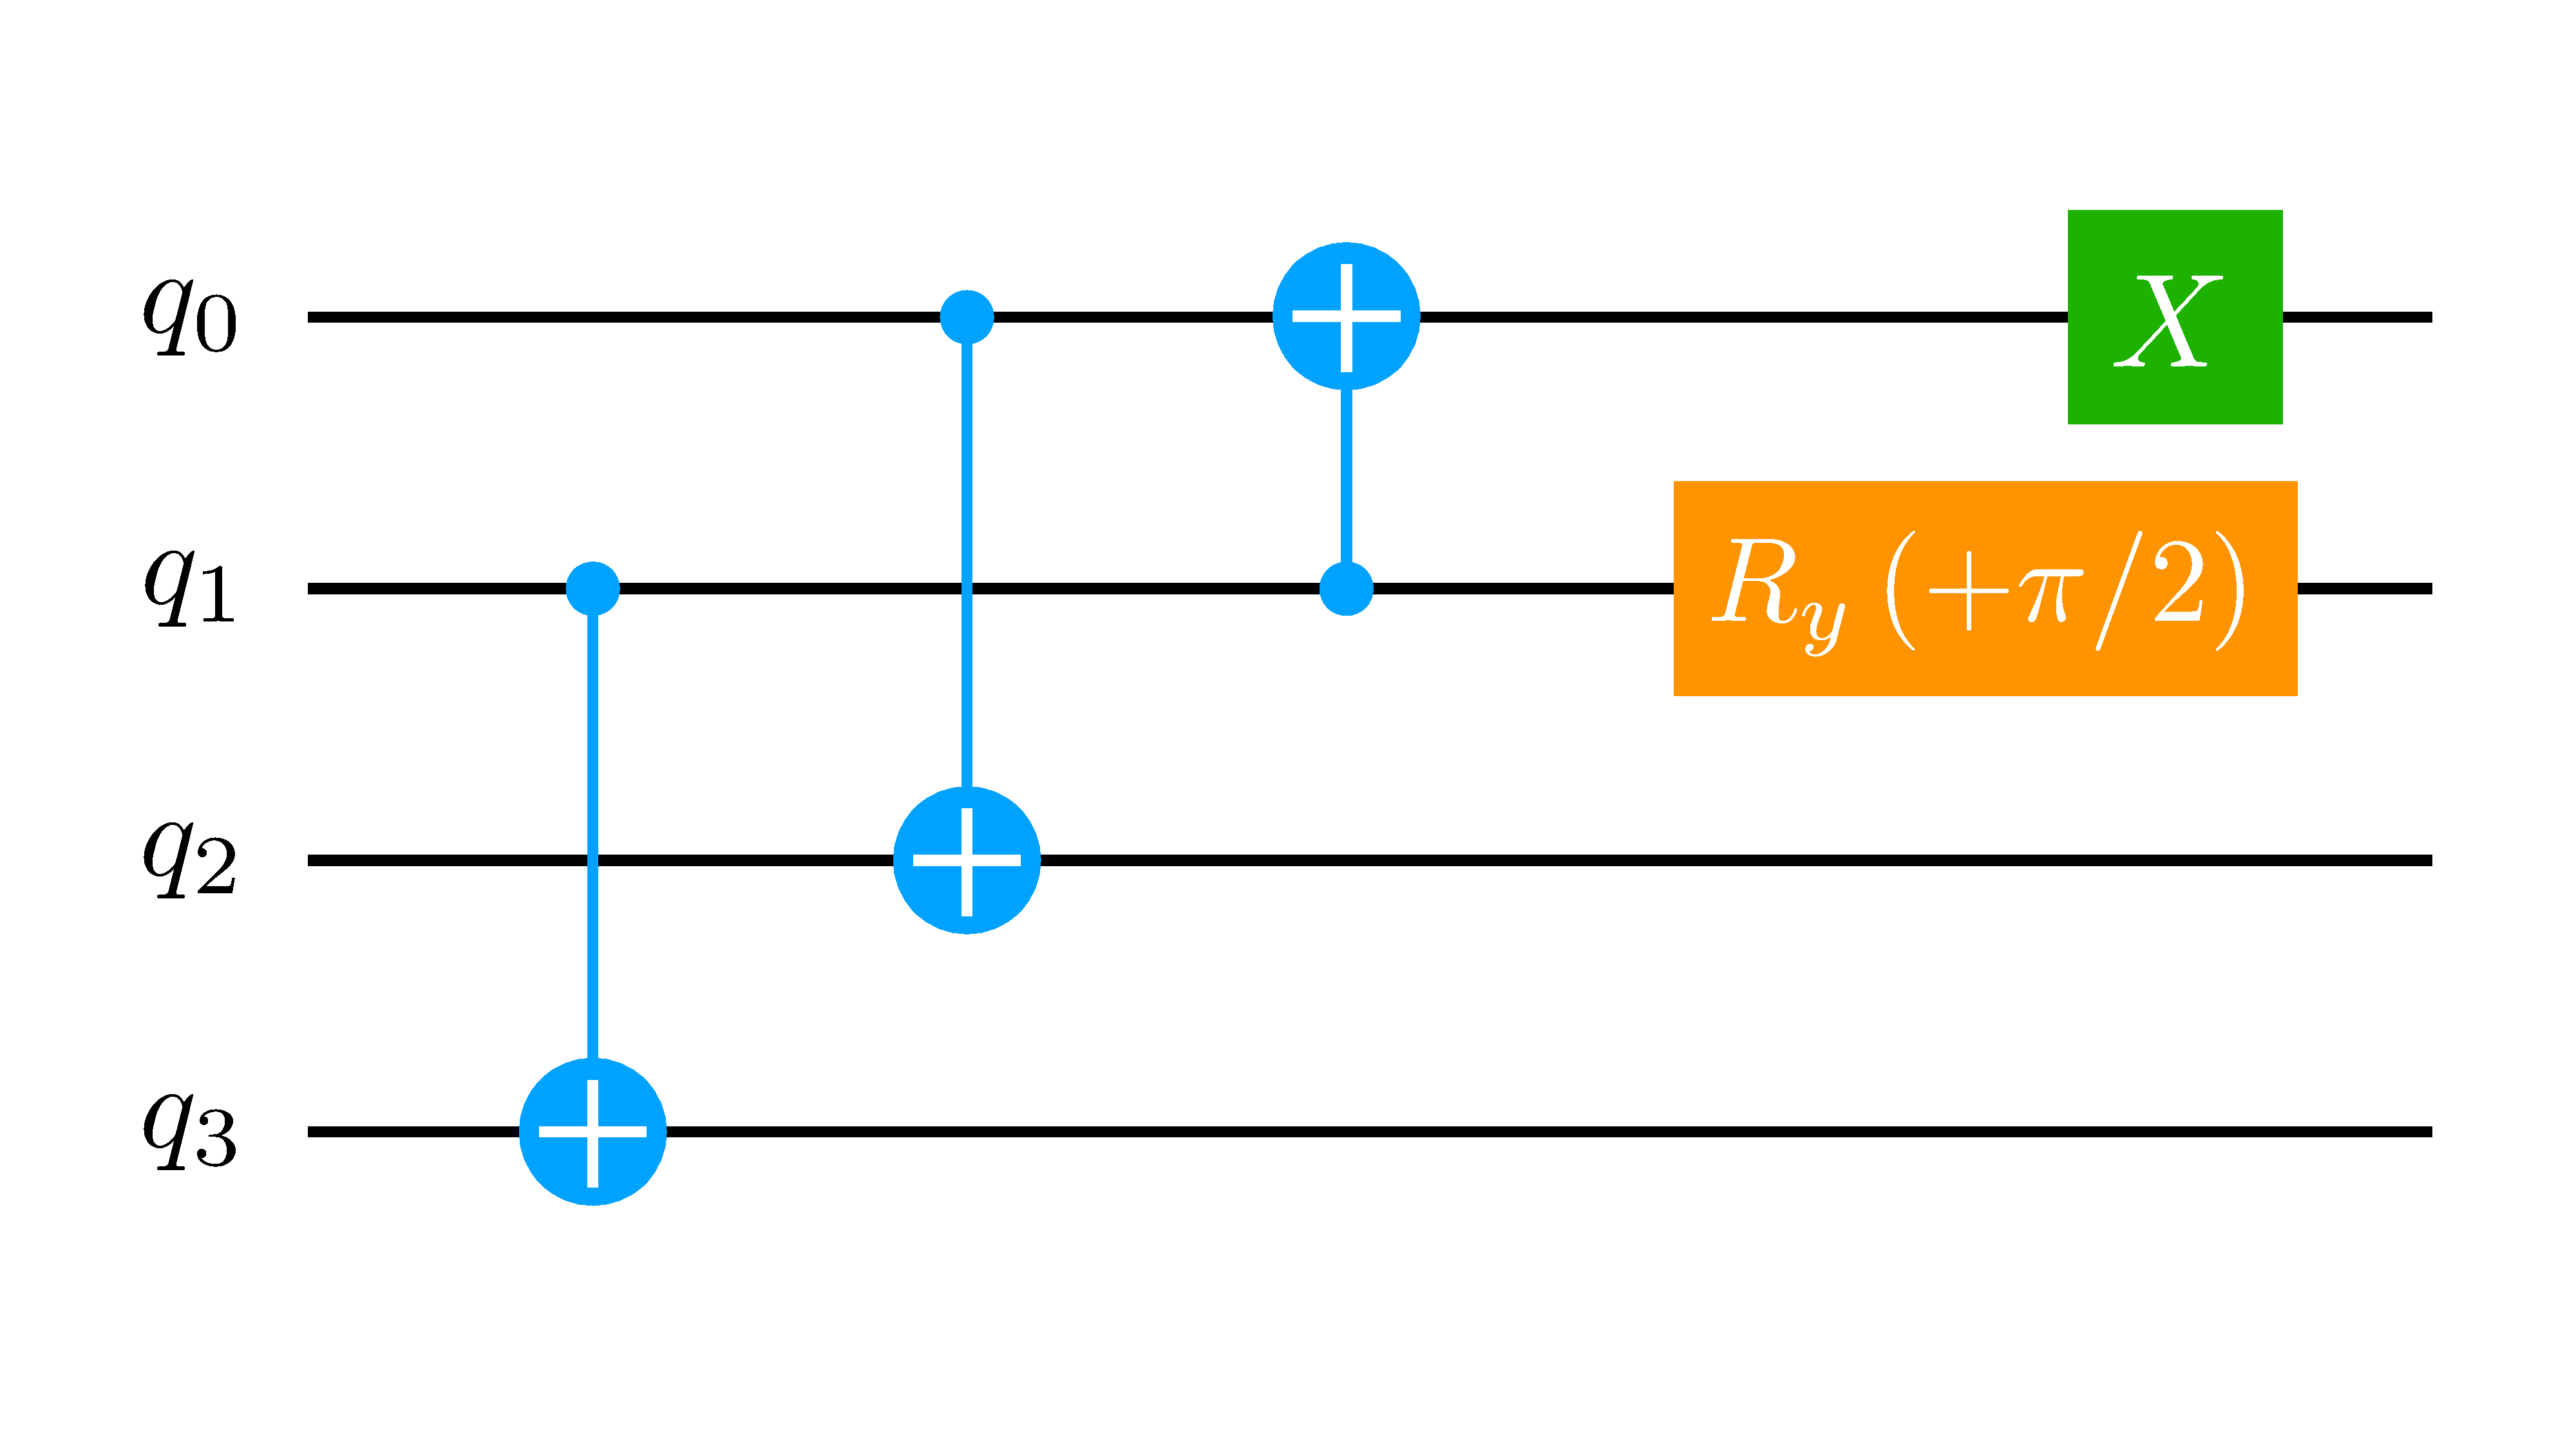
\includegraphics[width=\linewidth]{Figures/NJL1-model-solving/ansatz-implementation-base-state-reversing-gamma}
		\end{minipage}
		\caption{(Left) Preparation $\Gamma$ of state $\ket{\gamma}$. (Right) Quantum gate $\Gamma^{-1}$ for reversing state $\ket{\gamma}$.}
	\end{figure}

\break

	\begin{figure}[!p]
		\centering
		\begin{minipage}[c]{.45\linewidth}
			\centering
			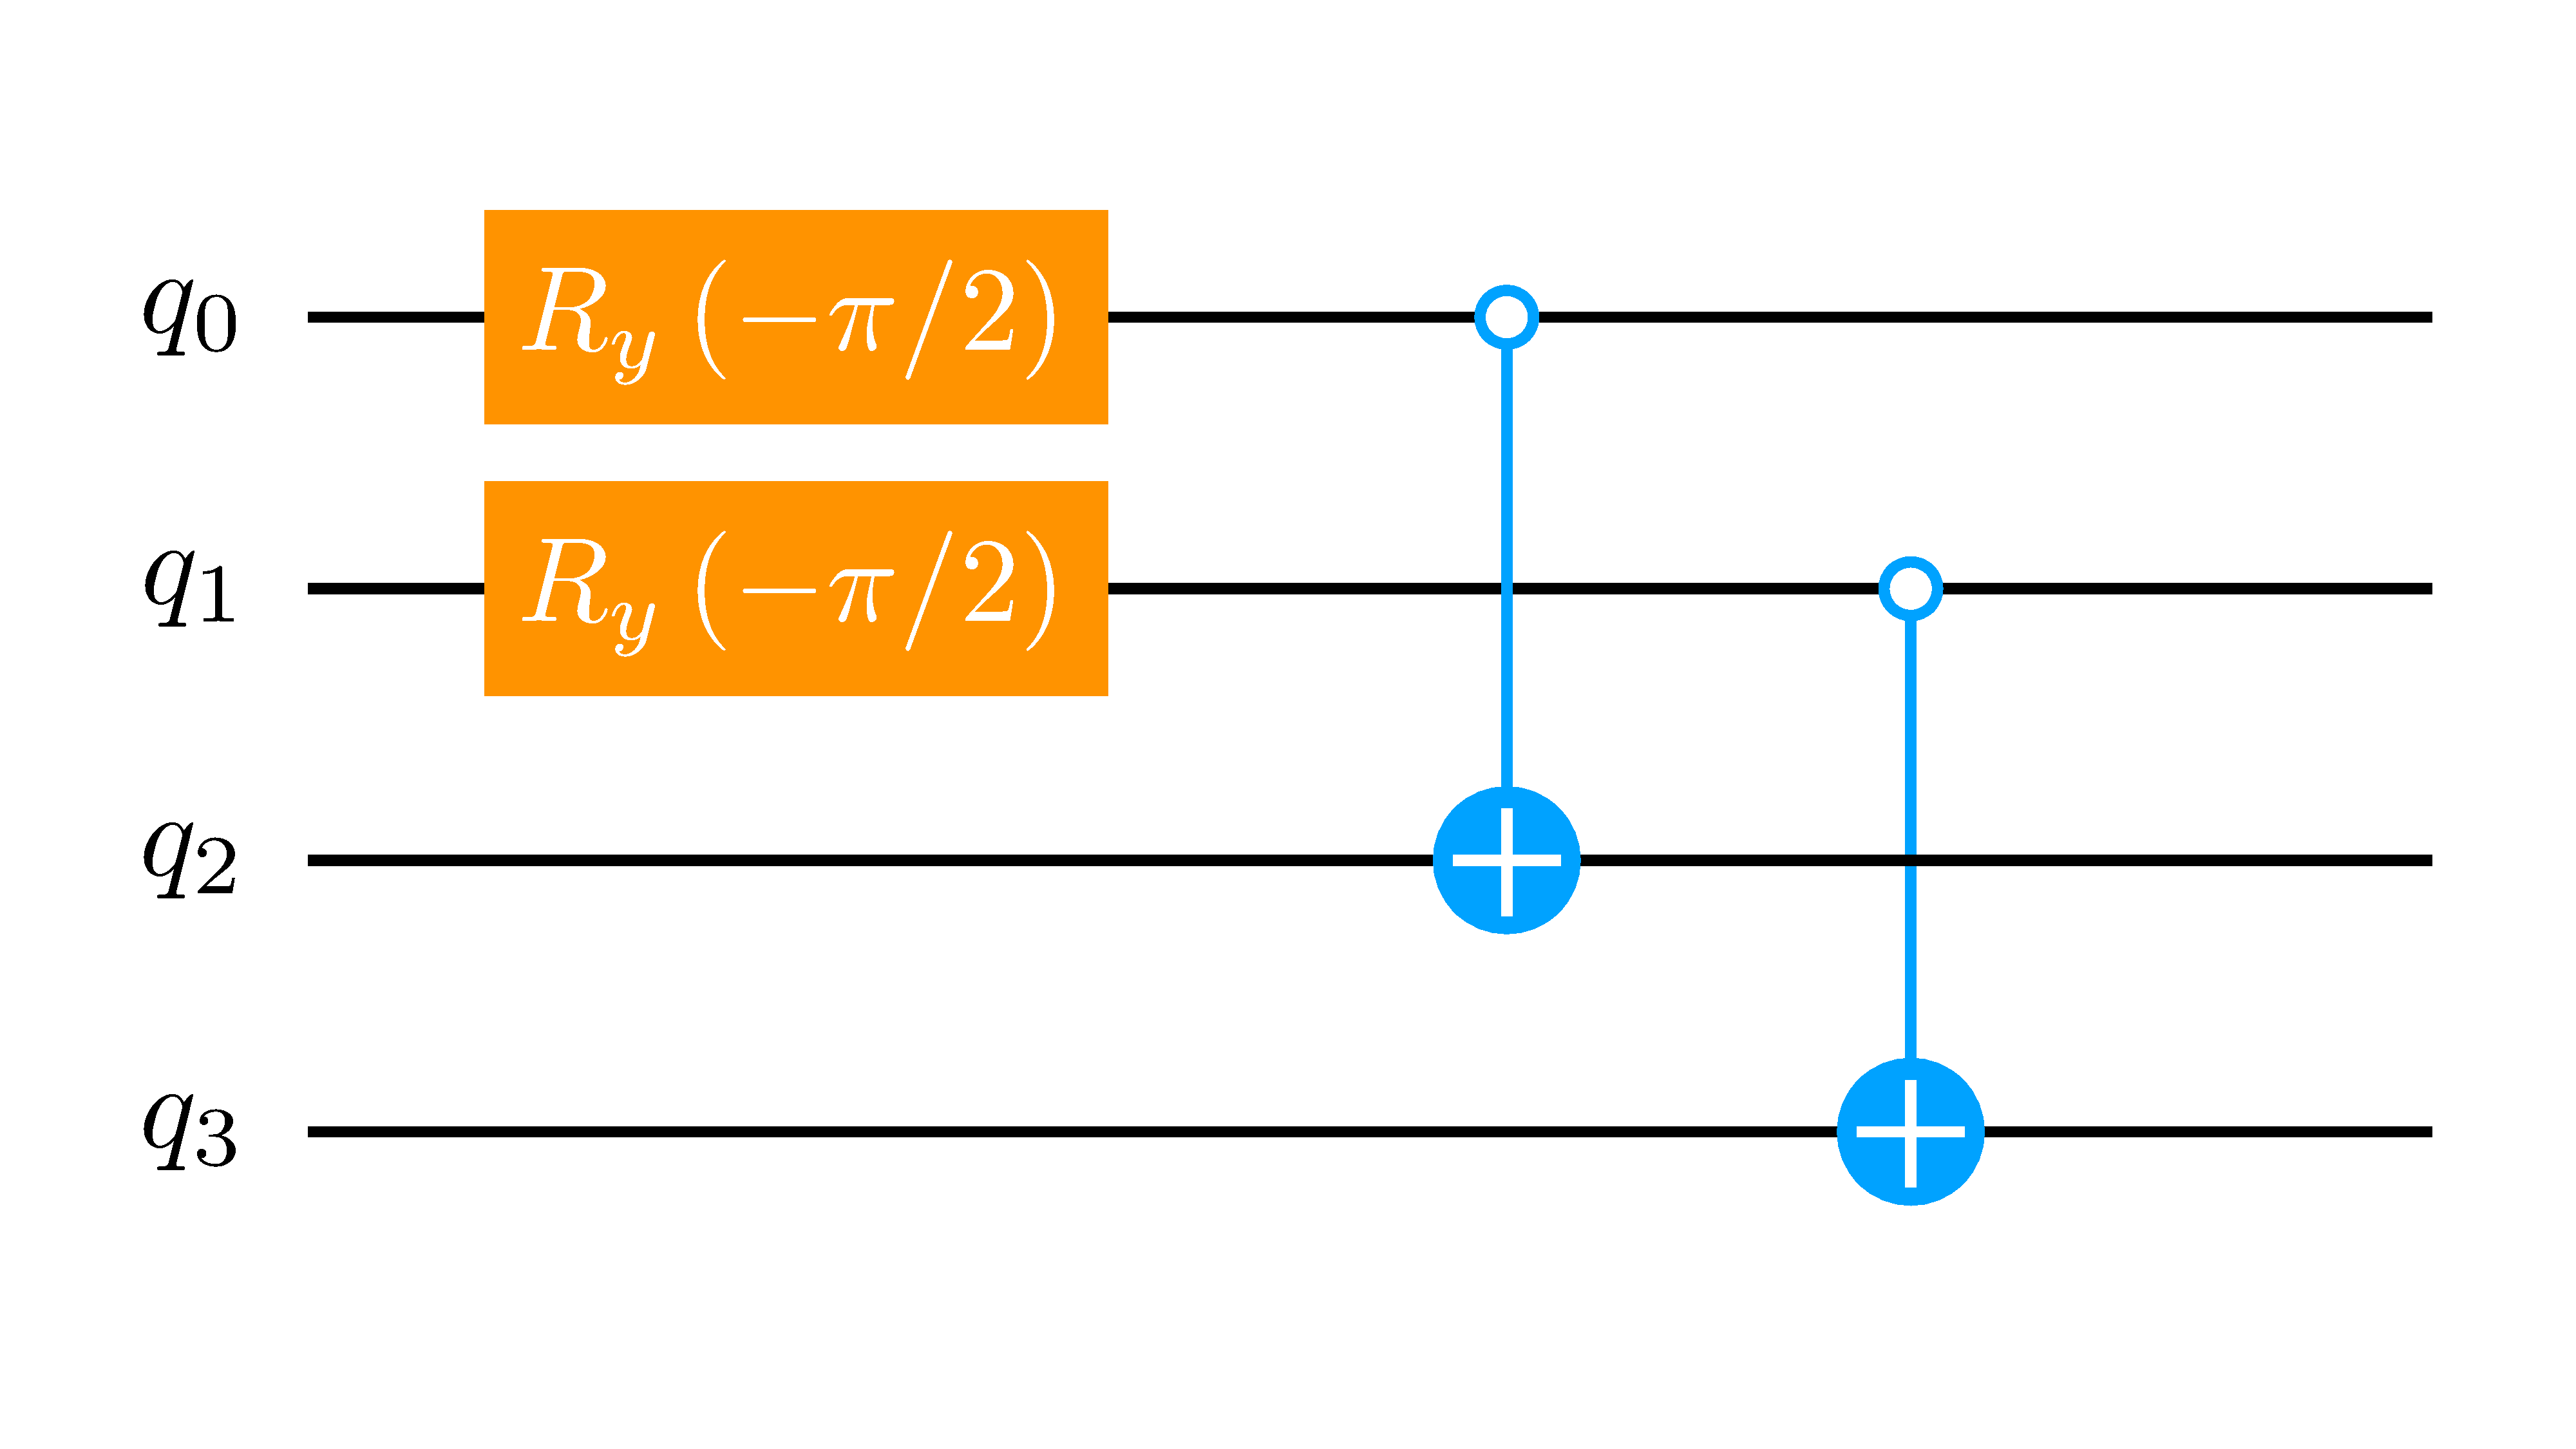
\includegraphics[width=\linewidth]{Figures/NJL1-model-solving/ansatz-implementation-base-state-preparation-kappa}
		\end{minipage}
	  \hspace{.025\linewidth}
		\begin{minipage}[c]{.45\linewidth}
			\centering
			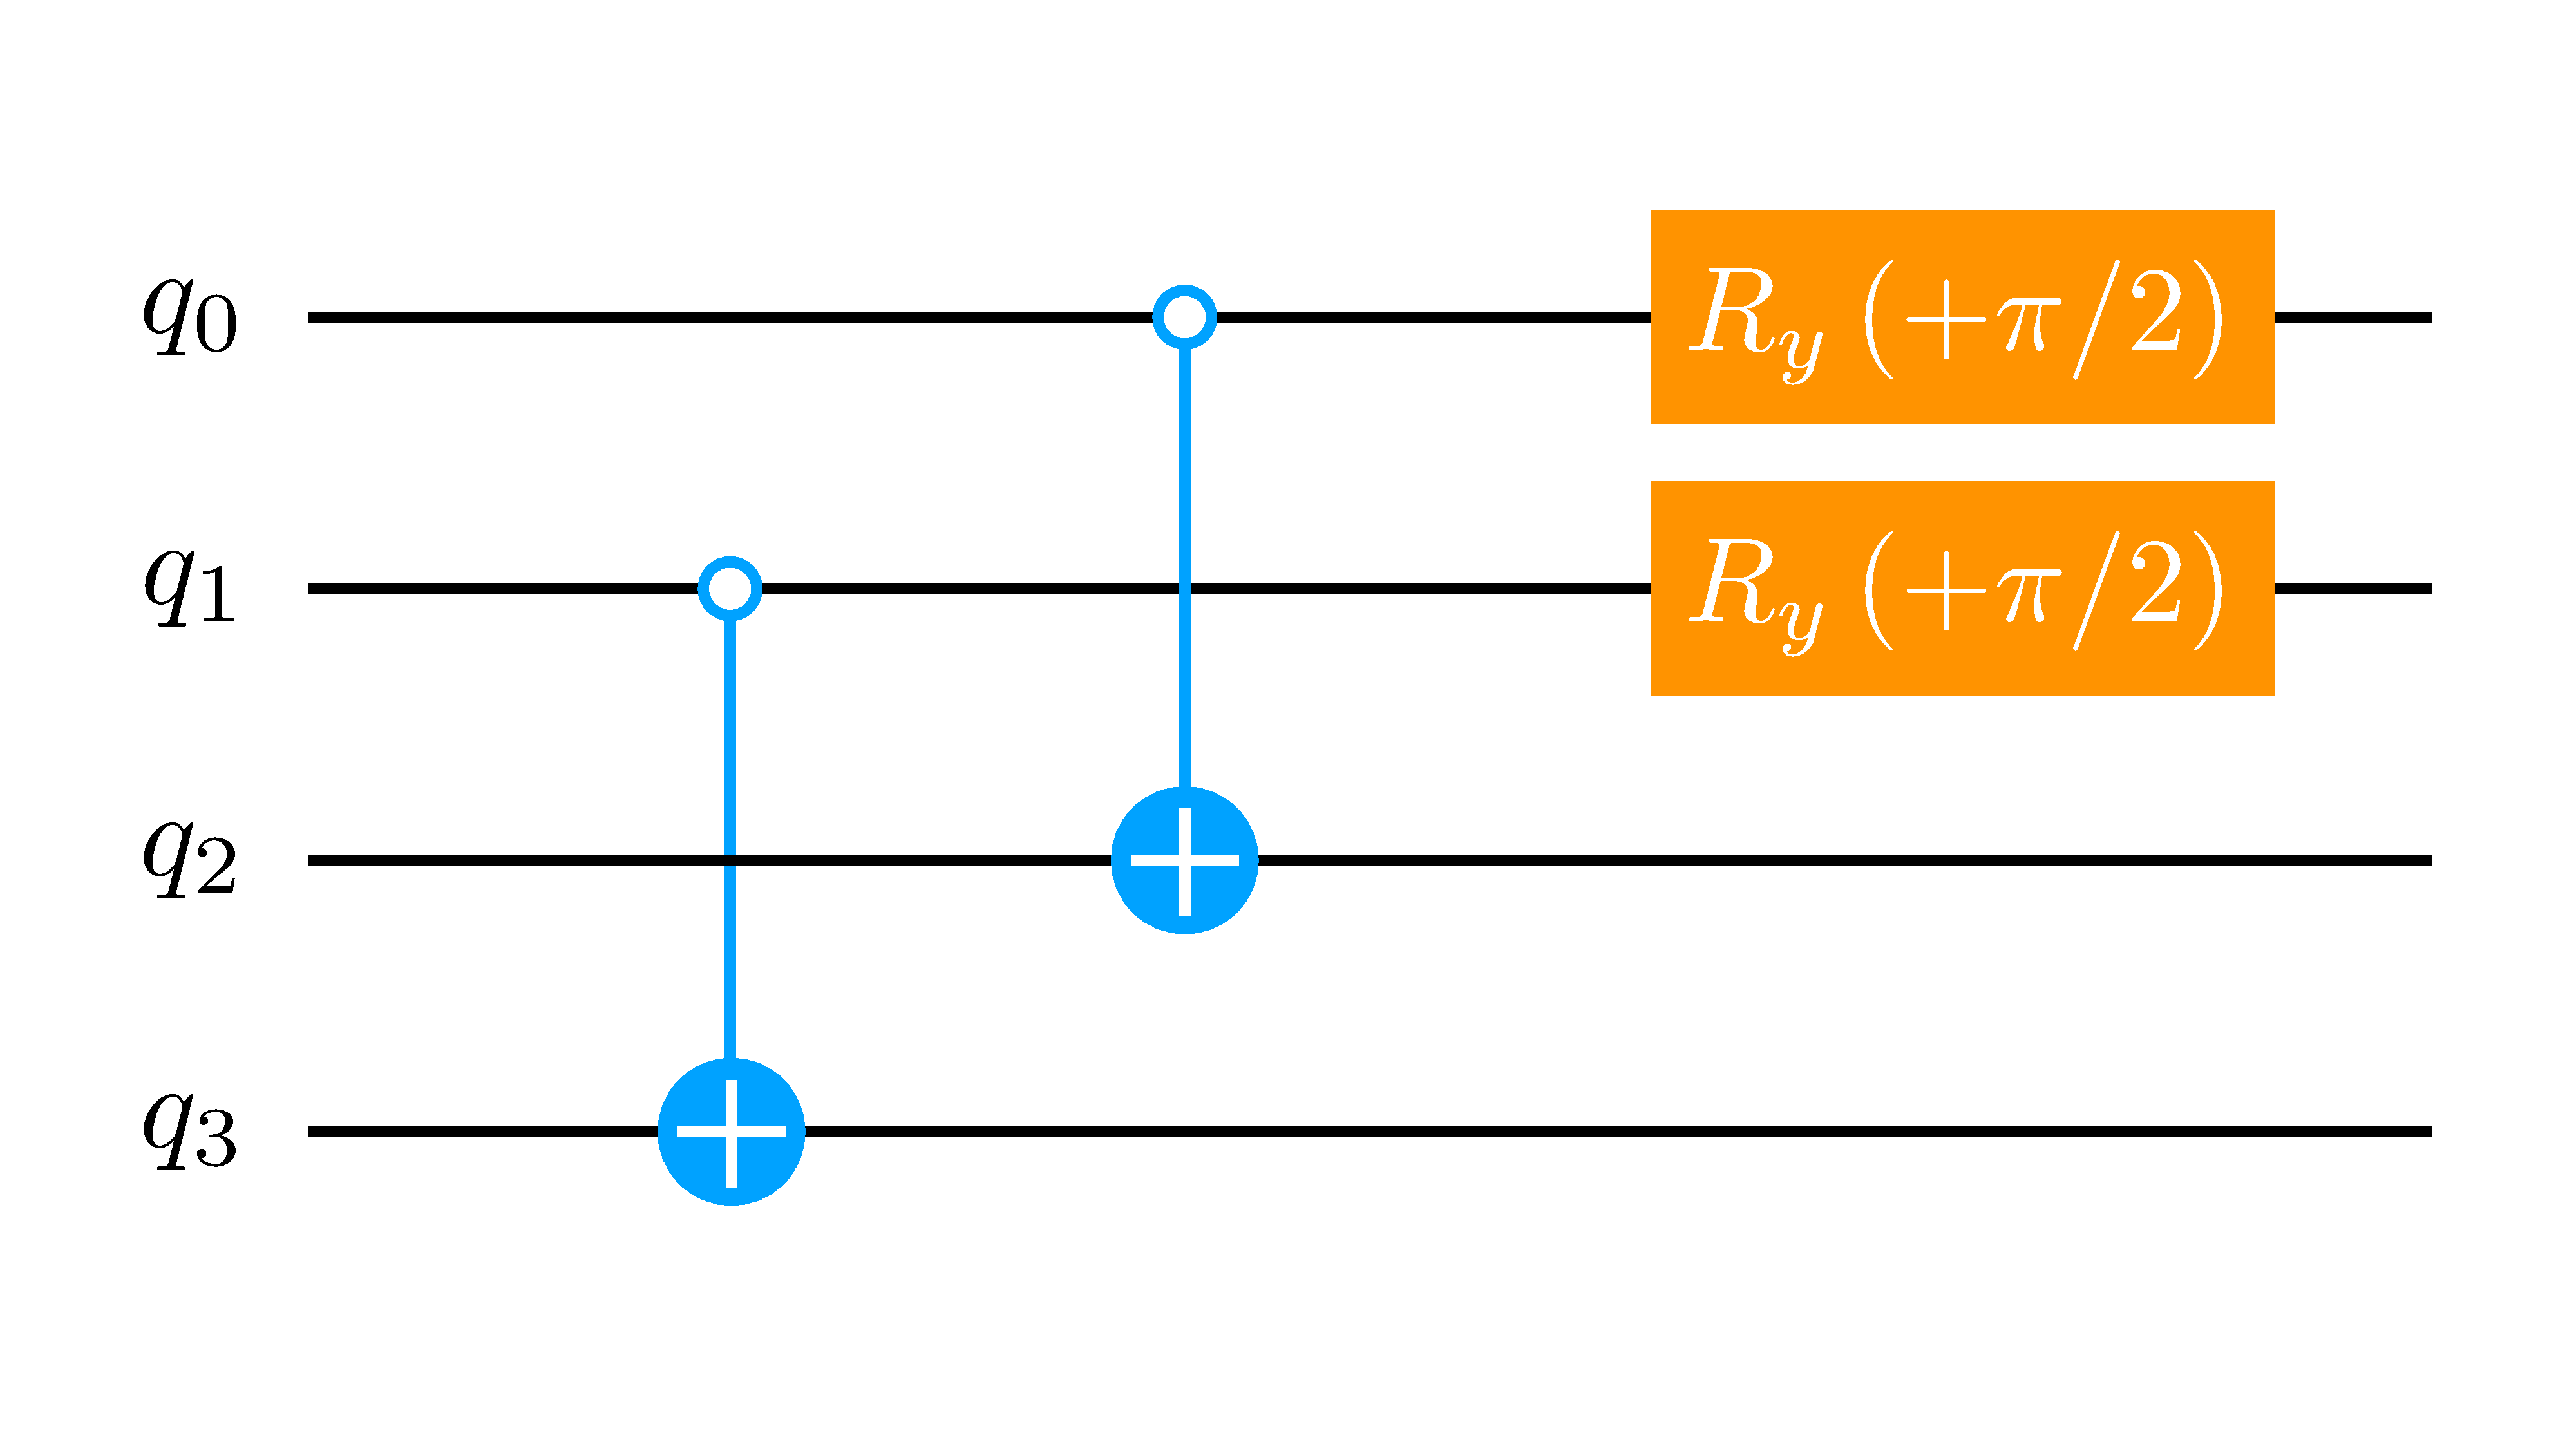
\includegraphics[width=\linewidth]{Figures/NJL1-model-solving/ansatz-implementation-base-state-reversing-kappa}
		\end{minipage}
		\caption{(Left) Preparation $\mathcal{K}$ of state $\ket{\kappa}$. (Right) Quantum gate $\mathcal{K}^{-1}$ for reversing state $\ket{\kappa}$.}
	\end{figure}


\end{frame}

%% ----------------------------------------------------------------------------

\begin{frame}[allowframebreaks]{Optimal sampling regression algorithm}

	The method that we have used to parametrize space will naturally return cycles in the the states that we are parametrizing. Such \textbf{periodic nature} will transfer to the expectation value function, which in turn allows us to consistently apply Fourier analysis to fully describe it:

	\begin{gather*}
	  f(\theta) \equiv a_0 + \sum_{s=1}^S \qty[a_s\cos(s\theta) + b_s\sin(s\theta)] \\
	  \mqty[
	    1 & \cos(\theta_1) & \sin(\theta_1) & \cos(2\theta_1)
	      & \cdots & \sin(S\theta_1) \\
	    1 & \cos(\theta_2) & \sin(\theta_2) & \cos(2\theta_2)
	      & \cdots & \sin(S\theta_2) \\
	    \vdots & \vdots & \vdots & \vdots & \ddots & \vdots \\
	    1 & \cos(\theta_{2S+1}) & \sin(\theta_{2S+1}) & \cos(2\theta_{2S+1})
	      & \cdots & \sin(S\theta_{2S+1})
	  ]
	  \mqty[
	    a_0 \\ a_1 \\ b_1 \\ a_2 \\ \vdots \\ b_S
	  ] =
	  \mqty[
	    f(\theta_1) \\ f(\theta_2) \\ \vdots \\ f(\theta_{2S+1})
	  ] \\[5pt]
	  Fc = f \qra F^{\dagger}Fc = F^{\dagger}f
	\end{gather*}

\break

	Generally $S \ra \infty$, however, if the bandwidth is bounded, $S$ will be finite and it will be possible to evaluate this expression exactly. Theoretically, the power of this method is demonstrated through the \textbf{Nyquist-Shannon sampling theorem}; which states that if a function $f(\theta)$ contains no angular frequencies higher than $\omega_{\text{S}}$, it is completely determined by giving its ordinates at a series of points $1/2\omega_{\text{S}}$ apart:

	\begin{gather*}
	  \omega_{\text{sampling}} > 2\omega_{\text{S}}
	\end{gather*}

	Extending these results to \textbf{higher dimensions} is straight forward considering multidimensional Fourier series. In this case, we may have a different bandwidth $S_{q}$ for each parameter. Calling the total number of parameters $Q$, and the maximum bandwidth $S_{\text{max}}$, the total number of samples $T$ required by this method is:

	\begin{gather*}
	  T = \prod_{q=1}^{Q} \qty(2 S_{q} + 1) = \order{S_{\text{max}}^{Q}}
	\end{gather*}

\end{frame}

%% ----------------------------------------------------------------------------
%% ----------------------------------------------------------------------------

\end{document}
